\part{Communication}

计算机在计算领域和通信领域都扮演着重要的角色,计算机之间的通信是通过计算机网络(Computer Network)实现的。计算机网络是为了通信和共享资源而以各种方式连在一起的一组计算设备,现在计算机网络也是一种基础设施,类似于复杂的高速公路系统,用各种方式把公路连接在一起,从而使汽车能够从出发点开到目的地。

计算机网络注重的是底层协议和数据传输率,通过计算机网络使数据能够从源计算机传送到目的计算机,接收数据的计算机的位置并不一定固定,但是当前地址是确定的。


\chapter{Network}

使用网络可以共享那些无形的资源(如文件)和有形的资源(如打印机)。Email、即时通信和网页都依赖于底层计算机网络中发生的通信。

计算机之间的连接通常是靠物理电线或电缆实现的,有些连接也可以使用无线电波或红外信号传导数据,这种连接是无线的,称为无线网络(Wireless Network)。

网络不是由物理连接定义的,而是由通信能力定义的。计算机网络中的设备不只是计算机,例如,打印机也可以直接连入网络,以便网络中的每个用户都可以使用它。此外,网络还包括各种处理网络信息传输的设备。我们用通用的术语节点(node)或主机(host)来引用网络中任何可寻址的设备。

计算机网络的一个关键问题是数据传输率(Data Transfer Rate),即数据从网络中的一个地点传输到另一个地点的速率。现在我们依靠网络传输更多更复杂(更大)的数据,比如多媒体等。

数据传输率又叫网络的带宽(Bandwidth)。在数据共享和传输过程中,网络固有的带宽限制定义了在固定时间内从一个地点传输到另一个地点的最大位数或字节数。

计算机网络的另一个关键问题是使用的协议(Protocol),协议说明了两个事物如何交互的一组规则,在计算术语中借用它来表示计算机在进行交互的时候使用的正确规定,或者说计算机网络通信协议是对那些计算机必须遵守以便彼此通信的的规则的描述。

计算机通信层的协议是一套规定必须严格遵守的规则和(交互信息的)过程的代码,在连网过程中,我们使用明确的协议来说明如何格式化和处理要传输的数据。

计算机网络开创了一个新的计算领域——客户/服务器模型(Client/Server Model)。计算机软件系统分布在整个网络中,在这个网络中,客户将向服务器请求信息或操作,服务器则对此做出响应。

例如,文件服务器(File Server)是网络中为多个用户存储和管理文件的计算机,这样每个用户不必都保存自己的文件副本。Web服务器(Web Server)是专用于响应(来自客户浏览器的)页面请求的计算机。现在,客户/服务器关系已经发展的非常复杂,而且客户/服务器模型在计算世界里也越来越重要了。

此外,现在客户/服务器模型除了支持基本的请求/响应功能之外,开始支持并行处理,即可以把一个问题分解为若干个小问题,然后用多台计算机来解决问题。使用计算机网络和客户/服务器模型,可以通过让客户请求多台机器执行一个问题的特定部分来实现并行处理,客户接收到每台机器的响应后,再把它们组合成一个完整的解决方案。

\section{Network Type}

计算机网络的分类方式有多种,通常根据网络的作用域对它们分类。局域网(Local Area Network,LAN)是连接较小地理范围的少量计算机的网络。LAN通常覆盖的是一个小的地理区域以及相对较少的互连设备,比如在一个房间或一幢建筑内,也可以延伸到几幢相邻的建筑中。管理LAN的各种配置叫做拓扑(Topology)。

环形拓扑(Ring Topology)把所有节点连接成一个封闭的环,消息在环中沿着一个方向传播。环形网络中的节点将传递消息,知道它们到达了目的地。星形拓扑(Star Topology)以一个节点为中心,其他节点都连接在中心节点上,所有消息都经过中心节点发送。星形网络给中心节点赋予了巨大的负荷,如果中心节点停止响应,那么整个网络的通信就瘫痪了。在总线拓扑(Bus Topology)中,所有节点都连接在一根通信线上,消息可以在通信线中双向传播。总线上的所有节点将检查总线传输的每个消息,不过如果消息所寻的地址不是该节点,它会忽略这条消息。以太网(Ethernet)的总线技术已经成为了局域网的业界标准。

\begin{figure}[!h]
\centering
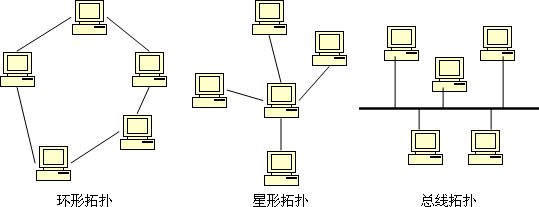
\includegraphics[scale=0.6]{network_topology.eps}
\caption{计算机网络拓扑}
\label{network_topology}
\end{figure}


广域网(Wide Area Network,WAN)是连接两个或多个相距较远的局域网的网络。网络之间的通信叫做网际互联,广域网使得较小的网络之间可以互相通信。

局域网中通常会有一个特殊节点作为网关(Gateway),处理当前局域网与其他网络之间的通信的就是网关。

\begin{figure}[!h]
\centering
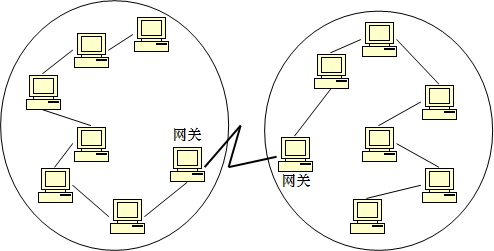
\includegraphics[scale=0.5]{network_gateway.png}
\caption{网关}
\label{network_gateway}
\end{figure}


城域网(Metropolitan Area Network,MAN),指的是在大城市内及其周边开发的基础通信设施,城域网络通常是采用创新技术(如光纤光缆)实现。


Internet本质上就是一个巨大的广域网,遍布整个地球,是所有的小网络的集合,这些小网络都采用相同的协议通信,而且会传递经过的消息,使它们能够到达最终目的地。

虽然术语Internet和Web常被混为一谈,但它们并不相同。万维网是分散在世界各处计算机上的信息和访问信息的软件构成的基础设施。而Web依靠底层网络(尤其是Internet)在用户之间交换信息。Web页不仅包含信息,还包含对其他资源(如图像等)的引用。由个人或公司管理的一组Web页叫做Web站点。全球各种Web页之间都有链接,这也是万维网这个名字的来源。




\section{Internet连接}


事实上,Internet(因特网)的概念,是1974年由温顿·瑟夫提出的。Internet作为一个广域网,它由多个小网络构成,这些小网络则通常属于某个人或某个公司,这些网络之间是如何连接的才真正定义了Internet,因此没有一个人或公司拥有Internet,甚至不能完整地控制它。


Internet骨干网(Internet Backbone)指的是承载Internet通信的一组高速网络。这些网络是由AT\&T、GTE和IBM这样的公司提供的。骨干网使用的是都是具有高数据传输率(从每秒1.5M到用特殊光缆实现的每秒600多兆位)的连接。

Internet服务提供者(Internet Service Provider,ISP)是给其他公司或个人提供Internet访问的公司,例如American Online等。ISP直接连接到Internet骨干网或者连接到更大的ISP。

把PC连接到Internet的方法有很多,最常用的三种方法是使用电话调制解调器、数字用户线路(DSL)或线缆调制解调器。

电话系统先于计算机网络进入千家万户,因此,以电话调制解调器作为家庭网络通信的首选方式就在情理之中。术语调制解调器(Modem)是调节器和解调器的缩写。


电话调制解调器将把计算机信息转换成模拟音频信号,以便在电话线中传输,目的地的调制解调器将把模拟音频信号转换回计算机信号。一种音频用于表示二进制的0,另一种用于表示1。

要使用电话调制解调器,必须首先将电脑与永久连接到Internet的计算机之间建立电话连接,而ISP就是通过这个连接来提供网络服务的。在给ISP付费后,就可以连接ISP提供的专用的计算机,建立连接后,就可以通过电话线把数据发送给ISP,ISP再把这些数据发送到Internet骨干网,传回的数据将被路由到你的ISP,最后发送到电脑上。

使用电话调制解调器不需要电话公司做任何特殊工作,而且数据被当作语音信号处理,所以除了在调制和解调的两端之外,不需要特殊的转换操作。


使用电话调制解调器连接的数据传输率被限制为模拟语音通信的数据传输率,最多每秒64Kbps。而如果把数据当作数字信号而不是模拟信号,那么电话线可以提供相当高的传输率,数字用户线路(Digital Subscriber Line,DSL)就是使用常规的铜质电话线传输数字信号的Internet连接方式。由于DSL和语音通信使用的频率不同,所以同一根电话线就可以满足这两种用途。


要建立DSL连接,首先电话公司要提供ISP服务,通过专门的计算机来处理数据通信。使用DSL,不必像电话调制解调器那样用拨电话的方式建立网络连接,DSL线路在PC与ISP之间维护了一个活动连接。不过由于数字信号在两点间传输的过程中会减弱,所以DSL传输速率会受到与ISP的专用计算机的距离的影响。


线缆调制解调器(Cable Modem)也是以数字形式来传输数据,不过采用的是有线电视信号的线缆,有线电视公司与ISP公司共享网络资源,提供线缆调制解调器的服务。

DSL连接和线缆调制解调器都属于宽带(Broadband)连接,即数据传输率至少为128Kbps,这两种方法提供的数据传输率都在每秒1.5M到3M之间。

DSL和线缆调制解调器的下载(Download)速度可以和上载(Upload)速度不同。


在 Internet 的早期,T1 连接被认为是非常快的连接。而今天的连接速度则要快得多。

在计算机网络中,1 字节等于 8 比特(这是用于传输一个字符的比特数),低速调制解调器能够传输大概 14 000 到 56 000 比特每秒(14 至 56 千比特每秒),即每秒传输 2000 至 7000 个字符,或大约 1 到 5 页文本。

一个千比特 (Kb) 是 1024 比特。一个兆比特 (Mb) 是 1024 千比特。一个 gigabit (Gb) 是 1024 兆比特。

下面是目前在 Internet 上被使用到的连接速度:

\begin{longtable}{|p{120pt}|p{120pt}|p{120pt}|}
%head
\multicolumn{3}{r}{}
\tabularnewline\hline
名称	&连接	&每秒的速度
\endhead
%endhead

%firsthead
\caption{Internet连接速度}\\
\hline
名称	&连接	&每秒的速度
\endfirsthead
%endhead

%foot
\multicolumn{3}{r}{}
\endfoot
%endfoot

%lastfoot
\endlastfoot
%endlastfoot
\hline
Modem		&Analog		&14.4-56Kb\\
\hline
D0			&Digital(ISDN)	&64Kb\\
\hline
T1			&Digital			&1.55Mb\\
\hline
T3			&Digital			&43Mb\\
\hline
OC-1		&Optical Carrier	&52Mb\\
\hline
OC-2		&Optical Carrier	&156Mb\\
\hline
OC-12		&Optical Carrier	&622Mb\\
\hline
OC-24		&Optical Carrier	&1.244Gb\\
\hline
OC-48		&Optical Carrier	&2.488Gb\\
\hline
\end{longtable}



\section{包交换}


ARPANET(阿帕网)作为全球互联网的鼻祖,第一次使用了报文交换技术,并且目前业已证实,该技术是由美国国防部高级研究计划局(DARPA)提供资金支持的。其设计初衷是,基于该技术建立的网络可用于各所大学与科研单位之间的相互交流,而不必担心网络连接不稳定问题。



但即便有国家国防部的资金投入,并不代表该项目必然与国防有所关联。同时,据项目负责人介绍,该项目更不会是出于躲避核袭击方面的考虑。鲍勃作为五角大楼的成员,当时也参与了该项目的运行,他表示ARPANET的设计动机决然和战争无关。



显然,没有阿帕网的建立,此后就没有互联网,更不要说预期利用网络覆盖达到抵御核攻击的宏伟目标了。事实上,对于阿帕网内部而言,关于分时性超级计算机的研发战略远比建立全球化军事网络为蓝图的战略部署要明确得多。




美国和英国的两个互联网研发小组,在大致相同的时间想到了报文交换技术。很多人认为,伦纳德和保尔在1969年发明了用以ARPANET的报文交换技术,但早在1965年,工作于英国国家物理研究室的研究员唐纳德便提交了分组交换的概念文档。


1967年,高级项目中介的项目管理经理约见了唐纳德,这两个不谋而合的研发小组自此开始强强联手,将成熟的报文交换技术最终用以ARPANET的建立。更有趣的是,报文交换技术是唐纳德最初的命名。

在20世纪70年代末,ARPANET上75\%以上的数据交换都来自于电子邮件(E-mail)。历史上第一封Email收信者和这封邮件的发出者都是同一个人,BBN公司(BroadBand Network)的网络工程师汤姆林森,他同时也是@这个邮箱符号的启用者。

为了提高在共享线路上传输信息的有效性,Internet上传输的消息被分割为大小固定、有编号的包(packet)。每个包将独立在网络上传输,直到到达目的地,它们将在此被重新组合为原始的消息,这种通信技术叫做包交换(Packet Switching)。

每个消息的包可以采用不同的路由线路,因此,它们到达目的地的顺序可能与发送顺序不同。需要把包按照正确顺序排列之后再组合成原始信息。


\begin{figure}[!h]
\centering
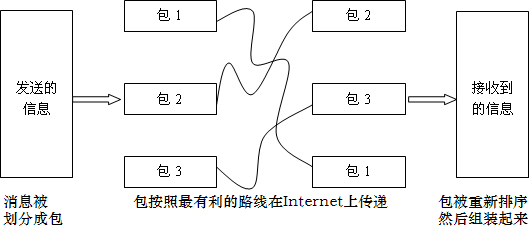
\includegraphics[scale=0.5]{network_pocket_switching.png}
\caption{包交换(Packet Switching)}
\label{network_pocket_switching}
\end{figure}

包在到达最终目的地之前,会在各种网络的计算机之间进行多次中转。用于指导包在网络之间传输的网络设备叫做路由器(Router)。中间的路由器不能规划包的整个传输路线,每个路由器只知道到达它的下一个目的地的最佳步骤。最终,消息将到达一个知道目的地机器的路由器。如果由于下行机器的问题中断了路径,或者选中的路径当前具有很大的通信量,那么路由器可能会把包发送给另一个路由器。

使用数字信号传输数据时,会有损失,使用中继器(Repeater)可以阻止这种情况发生。如果通信线路跨越的距离很长(如跨海的),那么线路上将安装中继器,以周期性地加强和传播信号。


\section{GPS}


GPS是全球定位系统(Global Positioning System)的缩写,即使用卫星技术查找25英尺之内的地点,这是一种用于确定方向的导航系统。


\chapter{Network Protocols}

计算机网络发展早期,不同的专有系统(Proprietary System)因为自己特有的差异导致不同类型的网络之间不能进行通信。

网络通信依靠协议支撑,由于这些原因(通常是历史原因),网络通信协议的大量出现,而且某些协议的地位比其他协议高。为了满足不同的网络之间互通信的需求,我们需要一种使不同的计算机系统能够通信的方式。


开放式系统(Open System)最大化了这种互通性(interoperability)的可能。


开放式系统的基础是一般的网络体系结构的通用模型和协议,它的实现采用了一系列协议,具有互通性。国际标准化组织ISO建立了开放式系统互连(OSI)参考模型来简化网络技术的开发。OSI参考模型在开放式系统的原则上把网络处理分成了7层,定义了一系列网络交互层,下面展示了OSI参考模型。

\begin{table}[!h]
\centering
\caption{OSI参考模型}
\label{Open_Systems_Interconnection_reference_model}
\begin{tabular}{|p{15pt}|p{80pt}|}
\hline
7	&应用层\\
\hline
6	&表示层\\
\hline
5	&会话层\\
\hline
4	&传输层\\
\hline
3	&网络层\\
\hline
2	&数据链路层\\
\hline
1	&物理层\\
\hline


\end{tabular}
\end{table}

开放式系统是以网络体系结构的通用模型为基础并且伴有一组协议的系统。开放式系统互连参考模型(Open Systems Interconnection reference model)是为了便于建立通信标准而对网络交互进行的7层逻辑划分。每一层处理网络通信的一个特定方面,最高层处理的是明确地与应用相关的问题。最低层处理的是与物理传输介质(如线型)相关的基础的电子或机械问题。其他层填补了其他各个方面,例如,网络层处理的是包的路由和寻址问题。之所以存在现在熟知的连网技术,都归功于开放式系统的技术和方法(如OSI参考模型)。






网络协议参照OSI参考模型的基本概念也进行了分层,以便OSI参考模型中的每一层都能依靠自己的基础协议,这样高层协议将以底层协议为支持。这种彼此依托的协议分层有时称为协议栈(Protocol Stack)。关键网络协议的分层示例如下:


\begin{figure}[!h]
\centering
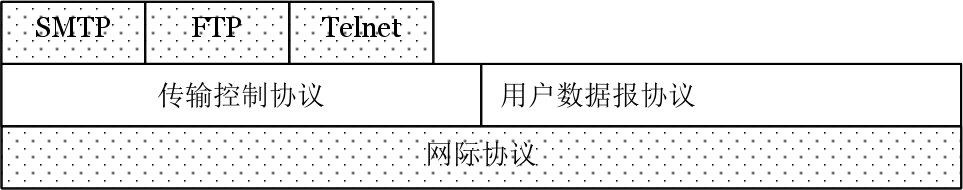
\includegraphics[scale=0.4]{network_protocol_stack.png}
\caption{协议栈(Protocol Stack)示例}
\label{network_protocol_stack}
\end{figure}


采用分层的方法,可以在不舍弃低层基础结构的前提下,开发新的协议。此外,这样还最小化了网络协议对网络处理其他方面的影响。有时,同一层中的协议提供同样的服务,但是采用的方式却不同。


上图中的最低两层构成了Internet通信的基础。其他协议有时叫做高层协议,负责处理特定类型的网络通信。这些层本质上是OSI参考模型的特定实现,以各种方式对应于该模型中的分层。


协议在某种意义上只是一种规约,规定了特定的数据类型必须按照特定的方式格式化,这些协议的重要之处在于它们提供了一种在连网的计算机之间进行交互的标准方式。文件格式的细节和数据域的大小对创建网络程序的开发者来说都是重要的。



\chapter{TCP/IP}


TCP/IP (Transmission Control Protocol / Internet Protocol)全称传输控制协议/网际协议\cite{tcp_ip},指的是一组协议和支持低层网络通信的工具程序,包含了一系列构成互联网基础的网络协议。

TCP/IP这种写法也反映了它们之间的关系,即TCP是在IP的基础之上的,同时也意味着TCP和IP在一起协同工作的,支持Internet通信的关键底层协议就是TCP/IP协议。



\section{History}


TCP/IP协议最早发源于美国国防部的ARPA网项目。TCP/IP模型也被称作DoD模型(Department of Defense Model)。TCP/IP字面上代表了两个协议:TCP(传输控制协议)和IP(网际协议)。

最初想到让不同电脑之间实现连接的,是美国加州大学洛杉矶分校网络工作小组的S.克罗克。1970年,克罗克及其小组着手制定最初的主机对主机通信协议,它被称为“网络控制协议”(NCP Network Control Protocol)。该协议被用于阿帕网,并在局部网络条件下运行稳定,但随着阿帕网用户的增多,NCP逐渐暴露出两大缺陷:

\begin{compactenum}
\item NCP只是一台主机对另一台主机的通讯协议,并未给网络中的每台电脑设置唯一的地址,结果就造成电脑在越来越庞大的网络中难以准确定位需要传输数据的对象。
\item NCP缺乏纠错功能,这样一来,数据在传输过程中一旦出现错误,网络就可能停止运行。出错电脑增多,使得网络运行效率大打折扣。
\end{compactenum}






最早的TCP/IP由文顿·瑟夫和罗伯特·卡恩两位开发,慢慢地通过竞争战胜了其他一些网络协议的方案,比如国际标准化组织ISO的OSI模型。TCP/IP的蓬勃发展发生在1990年代中期。当时一些重要而可靠的工具的出世,例如页面描述语言HTML和浏览器Mosaic,导致了互联网应用的飞速发展。

在构建了阿帕网先驱之后,DARPA开始了其他数据传输技术的研究。NCP诞生后两年,1972年,罗伯特·卡恩(Robert E. Kahn)被DARPA的信息技术处理办公室雇佣,在那里他研究卫星数据包网络和地面无线数据包网络,并且意识到能够在它们之间沟通的价值。在1973年春天,已有的ARPANET网络控制程序(NCP)协议的开发者文顿·瑟夫(Vinton Cerf)加入到卡恩为ARPANET设计下一代协议而开发开放互连模型的工作中。

到了1973年夏天,卡恩和瑟夫很快就开发出了一个基本的改进形式,其中网络协议之间的不同通过使用一个公用互联网络协议而隐藏起来,并且可靠性由主机保证而不是像ARPANET那样由网络保证。(瑟夫称赞Hubert Zimmerman和Louis Pouzin(CYCLADES网络的设计者)在这个设计上发挥了重要影响。)

由于网络的作用减少到最小的程度,就有可能将任何网络连接到一起,而不用管它们不同的特点,这样就解决了卡恩最初的问题。(一个流行的说法提到瑟夫和卡恩工作的最终产品TCP/IP将在运行“两个罐子和一根弦”上,实际上它已经用在信鸽上。一个称为网关(后来改为路由器以免与网关混淆)的计算机为每个网络提供一个接口并且在它们之间来回传输数据包。

这个设计思想更细的形式由瑟夫在斯坦福的网络研究组的1973年–1974年期间开发出来。(处于同一时期的诞生了PARC通用包协议组的施乐PARC早期网络研究工作也有重要的技术影响;人们在两者之间摇摆不定。)

DARPA于是与BBN、斯坦福和伦敦大学签署了协议开发不同硬件平台上协议的运行版本。有四个版本被开发出来——TCP v1、TCP v2、在1978年春天分成TCP v3和IP v3的版本,后来就是稳定的TCP/IP v4——目前因特网仍然使用的标准协议。

随着互联网的发展,目前流行的IPv4协议(网际协议版本四)已经接近它的功能上限。IPv4最致命的两个缺陷在于:

\begin{compactitem}
\item 地址只有32位,IP地址空间有限;
\item 不支持服务质量(Quality of Service,QoS)的想法,无法管理带宽和优先级,故而不能很好的支持现今越来越多的实时的语音和视频应用。因此IPv6(网际协议版本六)浮出水面,用以取代IPv4。
\end{compactitem}

1975年,两个网络之间的TCP/IP通信在斯坦福和伦敦大学(UCL)之间进行了测试。1977年11月,三个网络之间的TCP/IP测试在美国、英国和挪威之间进行。在1978年到1983年间,其他一些TCP/IP原型在多个研究中心之间开发出来。ARPANET完全转换到TCP/IP在1983年1月1日发生。

1983年1月1日,在因特网的前身(ARPA网)中,TCP/IP协议取代了旧的网络控制协议(NCP,Network Control Protocol),从而成为今天的互联网的基石。

1984年,美国国防部将TCP/IP作为所有计算机网络的标准。1985年,因特网架构理事会举行了一个三天有250家厂商代表参加的关于计算产业使用TCP/IP的工作会议,帮助协议的推广并且引领它日渐增长的商业应用。

2005年9月9日卡恩和瑟夫由于他们对于美国文化做出的卓越贡献被授予总统自由勋章。


TCP/IP成功的另一个因素在于对为数众多的低层协议的支持。这些低层协议对应OSI模型中的第一层(实体层)和第二层(数据链路层)。每层的所有协议几乎都有一半数量支持TCP/IP,例如:以太网(Ethernet)、令牌环(Token Ring)、光纤数据分布接口(FDDI)、端对端协议(PPP)、X.25、帧中继(Frame Relay)、ATM、Sonet、SDH等。

\section{Key Architectural Principles}



TCP/IP 是供已连接因特网的计算机进行通信的通信协议,通信协议是对计算机必须遵守的规则的描述,只有遵守这些规则,计算机之间才能进行通信。

整个通信网络的任务,可以划分成不同的功能区块,即所谓的层级(layer)。用于互联网的协议可以比照TCP/IP参考模型进行分类。TCP/IP协议栈起始于第三层协议IP(网际协议)。所有这些协议都在相应的RFC文档中讨论及标准化。重要的协议在相应的RFC文档中均标记了状态:“必须”(required),“推荐”(recommended),“可选”(elective)。其他的协议还可能有“试验”(experimental)或“历史”(historic)的状态。”



浏览器和服务器均使用 TCP/IP 来连接Internet。浏览器使用 TCP/IP 来访问服务器,服务器使用 TCP/IP 向浏览器传回 HTML,电子邮件程序也是使用 TCP/IP与Internet连接的,这样才能收发邮件。

\begin{compactitem}
\item TCP协议和软件负责把消息分割成包,交给IP软件传递,目的地机器上的TCP则负责把包排序,重新组合成信息,并负责处理错误。TCP软件还要处理所有发生的错误,如一个包永远不能到达目的地。

简单的说,TCP控制应用程序之间的通信。

\item IP协议和软件处理的是包通过互相连接的网络传递到最终目的地的路由选择,或者说,IP协议和软件负责包的路由,将包发送至接受者。

简单的说,IP控制计算机之间的通信。


\item UDP是用户数据报协议(User Datagram Protocol)的缩写,它是TCP的替代品,控制应用程序之间的简单通信。

简单的说,UDP软件的角色基本上与TCP软件一样,主要的不同之处在于TCP牺牲了一定的性能,提供了高度可靠性,而UDP更快,但不那么可靠。
\end{compactitem}

\begin{figure}[!ht]
\centering
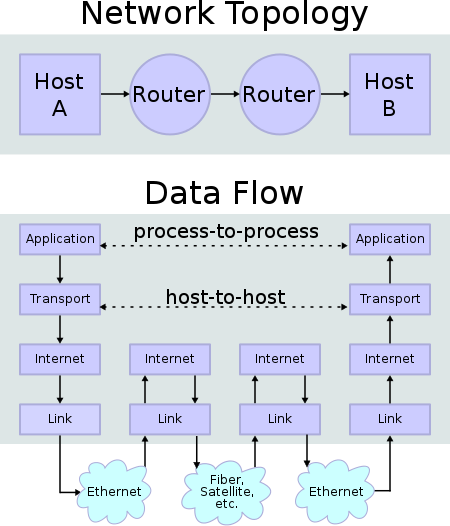
\includegraphics[scale=0.5]{IP_stack_connections.png}
\caption{两个因特网主机通过两个路由器和对应的层连接。各主机上的应用通过一些数据通道相互执行读取操作。}
\label{IP_stack_connections}
\end{figure}



UDP也是TCP/IP协议组的一部分,由于TCP是高度可靠的,还出于一定的历史原因,所以这套协议叫做TCP/IP协议。现在,TCP/IP被用来指称基于 TCP 和 IP 这两个最初的协议之上的不同的通信协议的大的集合(协议族),因特网地址\textcolor{Blue}{XXX.XXX.XXX.XXX}也是标准的 TCP/IP 协议的一部分。


所有的TCP/IP应用都必须实现IP和ICMP。对于一个路由器(router)而言,有这两个协议就可以运作了,虽然从应用的角度来看,这样一个路由器意义不大。实际的路由器一般还需要运行许多“推荐”使用的协议,以及一些其他的协议。

这样,TCP/IP 定义了电子设备(比如计算机)如何连入因特网,以及数据如何在它们之间传输的标准,其中:

\begin{compactitem}
\item TCP 使用固定的连接

当应用程序希望通过 TCP 与另一个应用程序通信时,它会发送一个通信请求。这个请求必须被送到一个确切的地址。在双方“握手”之后,TCP 将在两个应用程序之间建立一个全双工 (full-duplex) 的通信。

这个全双工的通信将占用两个计算机之间的通信线路,直到它被一方或双方关闭为止。UDP 和 TCP 很相似,但是更简单,同时可靠性低于 TCP。

\item IP 是无连接的

IP 是无连接的通信协议,它不会占用两个正在通信的计算机之间的通信线路。这样,IP 就降低了对网络线路的需求。每条线可以同时满足许多不同的计算机之间的通信需要。

通过 IP,消息(或者其他数据)被分割为小的独立的数据包,并通过因特网在计算机之间传送。在这个过程中,IP 负责将每个数据包路由至它的目的地。
\end{compactitem}

\zihao{6}

\begin{longtable}{|p{30pt}|p{110pt}|p{240pt}|}
%head
\multicolumn{3}{r}{}
\tabularnewline\hline
协议	& 名称 & 描述
\endhead
%endhead

%firsthead
\caption{网络通信协议集合}\\
\hline
协议	& 名称 & 描述
\endfirsthead
%endfirsthead

%foot
\multicolumn{3}{r}{}
\endfoot
%endfoot

%lastfoot
\endlastfoot
%endlastfoot
\hline
TCP		&传输控制协议						&TCP 用于从应用程序到网络的数据传输控制,负责在数据传送之前将它们分割为 IP 包,然后在它们到达的时候将它们重组。\\
\hline
IP		&网际协议							&IP 负责计算机之间的通信,负责在因特网上发送和接收数据包。\\
\hline
HTTP	&超文本传输协议						&HTTP 负责 web 服务器与 web 浏览器之间的通信,用于从 web 客户端(浏览器)向 web 服务器发送请求,并从 web 服务器向 web 客户端返回内容(网页)。\\
\hline
HTTPS	&安全的 HTTP						&HTTPS 负责在 web 服务器和 web 浏览器之间的安全通信。作为有代表性的应用,HTTPS 会用于处理信用卡交易和其他的敏感数据。\\
\hline
SSL		&安全套接字层						&SSL 协议用于为安全数据传输加密数据。\\
\hline
SMTP	&简易邮件传输协议					&SMTP 用于电子邮件的传输。\\
\hline
MIME	&多用途因特网邮件扩展				&MIME 协议使 SMTP 有能力通过 TCP/IP 网络传输多媒体文件,包括声音、视频和二进制数据。	\\
\hline
IMAP	&因特网消息访问协议					&IMAP 用于存储和取回电子邮件。\\
\hline
POP		&邮局协议							&POP 用于从电子邮件服务器向个人电脑下载电子邮件。\\
\hline
FTP		&文件传输协议						&FTP 负责计算机之间的文件传输。\\
\hline
NTP		&网络时间协议						&NTP 用于在计算机之间同步时间(钟)。\\
\hline
DHCP	&动态主机配置协议					&DHCP 用于向网络中的计算机分配动态 IP 地址。\\
\hline
SNMP	&简单网络管理协议					&SNMP 用于计算机网络的管理。\\
\hline
LDAP	&轻量级的目录访问协议				&LDAP 用于从因特网搜集关于用户和电子邮件地址的信息。\\
\hline
ICMP	&因特网消息控制协议					&ICMP 负责网络中的错误处理。\\
\hline
ARP		&Address Resolution Protocol			&ARP用于通过 IP 来查找基于 IP 地址的计算机网卡的硬件地址。\\
\hline
RARP	&Reverse Address Resolution Protocol	&RARP 用于通过 IP 查找基于硬件地址的计算机网卡的 IP 地址。\\
\hline
BOOTP	&Boot Protocol						&BOOTP 用于从网络启动计算机。\\
\hline
PPTP	&点对点隧道协议						&PPTP 用于私人网络之间的连接(隧道)。\\
\hline

\end{longtable}

\zihao{5}

其中:

\begin{compactitem}
\item 一个简单的路由器上可能会实现ARP,IP,ICMP,UDP,SNMP,RIP。
\item WWW用户端使用ARP,IP,ICMP,UDP,TCP,DNS,HTTP,FTP。
\item 一台用户电脑上还会运行如TELNET,SMTP,POP3,SNMP,ECHO,DHCP,SSH,NNTP。
\item 无盘设备可能会在固件,比如ROM中实现了ARP,IP,ICMP,UDP,BOOT,TFTP(均为面向数据包的协议,实现起来相对简单)。
\end{compactitem}


IP程序ping可以用于测试网络指派的可达性,即一台特定的网络计算机是否是活动的以及是否可到达,每个运行IP软件的计算机都会对ping请求做出回应,这使得ping成了一种方便的测试方式,无论特定的计算机是否在运行,也无论是否能通过网络达到它。

ping是Packet InterNet Groper的正式缩写,这个名称来源于潜水艇发送一个声纳脉冲,然后侦听返回的回声所采用的术语。由于ping是在IP层运行的,所以即使高层协议没有响应,它常常也会做出反应。

另一种TCP/IP工具叫做跟踪路由程序(traceroute),用于展示包在到达目的节点的过程中经过的路线,跟踪路由程序输出的是作为中转站的计算机的列表。


当一个 IP 包从一台计算机被发送,它会到达一个 IP 路由器。IP 路由器负责将这个包路由至它的目的地,直接地或者通过其他的路由器。

在一个相同的通信中,一个包所经由的路径可能会和其他的包不同。而路由器负责根据通信量、网络中的错误或者其他参数来进行正确地寻址。

几乎所有连接到互联网上的电脑上都存在的IPv4协议出生在1981年,今天的版本和最早的版本并没有多少改变。升级版IPv6的工作始于1995年,目的在于取代IPv4。ICMP协议主要用于收集有关网络的信息查找错误等工作。

\section{TCP/IP \& OSI}

TCP/IP参考模型是一个抽象的分层模型,这个模型中,所有的TCP/IP系列网络协议都被归类到4个抽象的"层"中。每一抽象层建立在低一层提供的服务上,并且为高一层提供服务。

完成一些特定的任务需要众多的协议协同工作,这些协议分布在参考模型的不同层中的,因此有时称它们为一个协议栈。

TCP/IP参考模型为TCP/IP协议栈订身制作。其中IP协议只关心如何使得数据能够跨越本地网络边界的问题,而不关心如何利用传输媒体,数据如何传输。整个TCP/IP协议栈则负责解决数据如何通过许许多多个点对点通路(一个点对点通路,也称为一``跳", 1 hop)顺利传输,由此不同的网络成员能够在许多``跳"的基础上建立相互的数据通路。

如想分析更普遍的网络通信问题,ISO的OSI模型也能起更好的帮助作用。

因特网协议族是一组实现支持因特网和大多数商业网络运行的协议栈的网络传输协议。它有时也被称为TCP/IP协议组,这个名称来源于其中两个最重要的协议:传输控制协议(TCP)和因特网协议(IP),它们也是最先定义的两个协议。

同许多其他协议一样网络传输协议也可以看作一个多层组合,每层解决数据传输中的一组问题并且向使用这些低层服务的高层提供定义好的服务。高层逻辑上与用户更为接近,所处理数据更为抽象,它们依赖于低层将数据转换成最终能够进行实体控制的形式。

网络传输协议能够大致匹配到一些厂商喜欢使用的固定7层的OSI模型。然而这些层并非都能够很好地与基于ip的网络对应(根据应用的设计和支持网络的不同它们确实是涉及到不同的层)并且一些人认为试图将因特网协议组对应到OSI会带来混淆而不是有所帮助。


\section{Internet Protocols Layers}

人们已经进行了一些讨论关于如何将TCP/IP参考模型映射到OSI模型。由于TCP/IP和OSI模型组不能精确地匹配,还没有一个完全正确的答案。

另外,OSI模型下层还不具备能够真正占据真正层的位置的能力;在传输层和网络层之间还需要另外一个层(网络互连层)。特定网络类型专用的一些协议应该运行在网络层上,但是却运行在基本的硬件帧交换上。类似协议的例子有地址解析协议和生成树协议(用来保持冗余网桥的空闲状态直到真正需要它们)。然而,它们是本地协议并且在网络互连功能下面运行。不可否认,将两个组(更不用说它们只是运行在如ICMP等不同的互连网络协议上的逻辑上的网络层的一部分)整个放在同一层会引起混淆,但是OSI模型还没有复杂到能够做更好的工作。


下面的图表试图显示不同的TCP/IP和其他的协议在最初OSI模型中的位置:



\begin{table}[!htbp]
\centering
\rowcolors{1}{White}{Lavender}
\begin{tabular}{l|l|l|}
\cline{2-3}
7&应用层&{\small HTTP,SMTP,SNMP,FTP,Telnet,SIP,SSH,NFS,RTSP,XMPP,Whois,ENRP等}\\ 
6&表示层&{\small XDR,ASN.1,SMB,AFP,NCP等}\\ 
5&会话层&{\small ASAP,SSH,ISO 8327/CCITT X.225,RPC,NetBIOS,ASP,Winsock,BSD sockets等}\\ 
4&传输层&{\small TCP,UDP,TLS,RTP,SCTP,SPX,ATP,IL等}\\ 
3&网络层&{\small IP,ICMP,IGMP,IPX,BGP,OSPF,RIP,IGRP,EIGRP,ARP,RARP,X.25等}\\ 
2&数据链路层&{\small 以太网,令牌环,HDLC,帧中继,ISDN,ATM,IEEE 802.11,FDDI,PPP等}\\ 
1&实体层&{\small 线路,无线电,光纤等}\\ \cline{2-3}
\end{tabular}
\end{table}


通常人们认为OSI模型的最上面三层(应用层、表示层和会话层)在TCP/IP组中是一个应用层。由于TCP/IP有一个相对较弱的会话层,由TCP和RTP下的打开和关闭连接组成,并且在TCP和UDP下的各种应用提供不同的端口号,这些功能能够被单个的应用程序(或者那些应用程序所使用的库)增加。与此相似的是,IP是按照将它下面的网络当作一个黑盒子的思想设计的,这样在讨论TCP/IP的时候就可以把它当作一个独立的层。

\begin{table}[!ht]
\centering
\rowcolors{1}{White}{Lavender}
\begin{tabular}{m{10pt}|m{60pt}|m{310pt}|}
\cline{2-3}
4&{\footnotesize 应用层\newline (OSI 5到7层)}&{\footnotesize 例如HTTP,FTP,DNS(如BGP和RIP这样的路由协议,尽管由于各种各样的原因它们分别运行在TCP和UDP上,仍然可以将它们看作网络层的一部分)}\\
3&{\footnotesize 传输层\newline (OSI 4层)}&{\footnotesize 例如TCP,UDP,RTP,SCTP(如OSPF这样的路由协议,尽管运行在IP上也可以看作是网络层的一部分)}\\
2&{\footnotesize 网络互连层\newline (OSI 3层)}&{\footnotesize 对于TCP/IP来说这是因特网协议(IP)(如ICMP和IGMP这样的必须协议尽管运行在IP上,也仍然可以看作是网络互连层的一部分;ARP不运行在IP上)}\\
1&{\footnotesize 网络接口层\newline (OSI 1和2层)}&{\footnotesize 例如以太网,Wi-Fi,MPLS等。}\\ \cline{2-3}
\end{tabular}
\end{table}


\subsection{应用层}


该层包括所有和应用程序协同工作,利用基础网络交换应用程序专用的数据的协议。 应用层是大多数普通与网络相关的程序为了通过网络与其他程序通信所使用的层。这个层的处理过程是应用特有的;数据从网络相关的程序以这种应用内部使用的格式进行传送,然后被编码成标准协议的格式。

一些特定的程序被认为运行在这个层上。它们提供服务直接支持用户应用。这些程序和它们对应的协议包括HTTP(万维网服务)、FTP(文件传输)、SMTP(电子邮件)、SSH(安全远程登陆)、DNS(名称<-> IP地址寻找)以及许多其他协议。
一旦从应用程序来的数据被编码成一个标准的应用层协议,它将被传送到IP栈的下一层。

在传输层,应用程序最常用的是TCP或者UDP,并且服务器应用程序经常与一个公开的端口号相联系。服务器应用程序的端口由互联网号码分配局(IANA)正式地分配,但是现今一些新协议的开发者经常选择它们自己的端口号。由于在同一个系统上很少超过少数几个的服务器应用,端口冲突引起的问题很少。应用软件通常也允许用户强制性地指定端口号作为运行参数。

连结外部的客户端程序通常使用系统分配的一个随机端口号。监听一个端口并且通过服务器将那个端口发送到应用的另外一个副本以建立对等连结(如IRC上的dcc文件传输)的应用也可以使用一个随机端口,但是应用程序通常允许定义一个特定的端口范围的规范以允许端口能够通过实现网络地址转换(NAT)的路由器映射到内部。

每一个应用层(TCP/IP参考模型的最高层)协议一般都会使用到两个传输层协议之一: 面向连接的TCP传输控制协议和无连接的包传输的UDP用户数据报文协议。

常用的应用层协议有:

\begin{compactitem}
\item 运行在TCP协议上的协议:

	\begin{compactitem}
	\item HTTP(Hypertext Transfer Protocol,超文本传输协议),主要用于普通浏览。
	\item HTTPS(Hypertext Transfer Protocol over Secure Socket Layer, or HTTP over SSL,安全超文本传输协议),HTTP协议的安全版本。
	\item FTP(File Transfer Protocol,文件传输协议),由名知义,用于文件传输。
	\item POP3(Post Office Protocol, version 3,邮局协议),收邮件用。
	\item SMTP(Simple Mail Transfer Protocol,简单邮件传输协议),用来发送电子邮件。
	\item TELNET(Teletype over the Network,网络电传),通过一个终端(terminal)登陆到网络。
	\item SSH(Secure Shell,用于替代安全性差的TELNET),用于加密安全登陆用。
	\end{compactitem}
\item 运行在UDP协议上的协议:
	\begin{compactitem}
	\item BOOTP(Boot Protocol,启动协议),应用于无盘设备。
	\item NTP(Network Time Protocol,网络时间协议),用于网络同步。
	\end{compactitem}
\item 其他:
	\begin{compactitem}
	\item DNS(Domain Name Service,域名服务),用于完成地址查找,邮件转发等工作(运行在TCP和UDP协议上)。
	\item ECHO(Echo Protocol,回绕协议),用于查错及测量应答时间(运行在TCP和UDP协议上)。
	\item SNMP(Simple Network Management Protocol,简单网络管理协议),用于网络信息的收集和网络管理。
	\item DHCP(Dynamic Host Configuration Protocol,动态主机配置协议),动态配置IP地址。
	\item ARP(Address Resolution Protocol,地址解析协议),用于动态解析以太网硬件的地址。
	\end{compactitem}
\end{compactitem}





\subsection{传输层}

传输层的协议,能够解决诸如端到端可靠性(“数据是否已经到达目的地?”)和保证数据按照正确的顺序到达这样的问题。在TCP/IP协议组中,传输协议也包括所给数据应该送给哪个应用程序。

在TCP/IP协议组中技术上位于这个层的动态路由协议通常被认为是网络层的一部分;一个例子就是OSPF(IP协议89)。

TCP(IP协议6)是一个“可靠的”、面向连结的传输机制,它提供一种可靠的字节流保证数据完整、无损并且按顺序到达。TCP尽量连续不断地测试网络的负载并且控制发送数据的速度以避免网络过载。另外,TCP试图将数据按照规定的顺序发送。这是它与UDP不同之处,这在实时数据流或者路由高网络层丢失率应用的时候可能成为一个缺陷。

较新的SCTP也是一个“可靠的”、面向连结的传输机制。它是面向纪录而不是面向字节的,它在一个单独的连结上提供了通过多路复用提供的多个子流。它也提供了多路自寻址支持,其中连结终端能够被多个IP地址表示(代表多个实体接口),这样的话即使其中一个连接失败了也不中断。它最初是为电话应用开发的(在IP上传输SS7),但是也可以用于其他的应用。

UDP(IP协议号17)是一个无连结的数据报协议。它是一个“尽力传递”(best effort)或者说“不可靠”协议——不是因为它特别不可靠,而是因为它不检查数据包是否已经到达目的地,并且不保证它们按顺序到达。如果一个应用程序需要这些特性,那它必须自行检测和判断,或者使用TCP协议。

UDP的典型性应用是如流媒体(音频和视频等)这样按时到达比可靠性更重要的应用,或者如DNS查找这样的简单查询/响应应用,如果建立可靠的连结所作的额外工作将是不成比例地大。

DCCP目前正由IEFT开发。它提供TCP流动控制语义,但对于用户来说保留了UDP的数据报服务模型。

TCP和UDP都用来支持一些高层的应用。任何给定网络地址的应用通过它们的TCP或者UDP端口号区分。根据惯例使一些大众所知的端口与特定的应用相联系。

RTP是为如音频和视频流这样的实时数据设计的数据报协议。RTP是使用UDP包格式作为基础的会话层,然而据说它位于因特网协议栈的传输层。




\subsection{网络互连层}

正如最初所定义的,网络层解决在一个单一网络上传输数据包的问题。类似的协议有X.25和ARPANET的Host/IMP Protocol。

随着因特网思想的出现,在这个层上添加了附加的功能,也就是将数据从源网络传输到目的网络。这就牵涉到在网络组成的网上选择路径将数据包传输,也就是因特网。

在因特网协议组中,IP完成数据从源发送到目的的基本任务。IP能够承载多种不同的高层协议的数据;这些协议使用一个唯一的IP协议号进行标识。ICMP和IGMP分别是1和2。

一些IP承载的协议,如ICMP(用来发送关于IP发送的诊断信息)和IGMP(用来管理多播数据),它们位于IP层之上但是完成网络层的功能,这表明了因特网和OSI模型之间的不兼容性。所有的路由协议,如BGP、OSPF、和RIP实际上也是网络层的一部分,尽管它们似乎应该属于更高的协议栈。






\subsection{网络接口层}



网络接口层实际上并不是因特网协议组中的一部分,但是它是数据包从一个设备的网络层传输到另外一个设备的网络层的方法。这个过程能够在网卡的软件驱动程序中控制,也可以在韧体或者专用芯片中控制。这将完成如添加报头准备发送、通过实体媒介实际发送这样一些数据链路功能。另一端,链路层将完成数据帧接收、去除报头并且将接收到的包传到网络层。

然而,链路层并不经常这样简单。它也可能是一个虚拟专有网络(VPN)或者隧道,在这里从网络层来的包使用隧道协议和其他(或者同样的)协议组发送而不是发送到实体的接口上。VPN和隧道通常预先建好,并且它们有一些直接发送到实体接口所没有的特殊特点(例如,它可以加密经过它的数据)。由于现在链路“层”是一个完整的网络,这种协议组的递归使用可能引起混淆。但是它是一个实现常见复杂功能的一个优秀方法。(尽管需要注意预防一个已经封装并且经隧道发送下去的数据包进行再次地封装和发送)。










在长期的发展过程中,IP逐渐取代其他网络。这里是一个简单的解释。IP传输通用数据。数据能够用于任何目的,并且能够很轻易地取代以前由专有数据网络传输的数据。下面是一个普通的过程:

\begin{compactenum}
\item 一个专有的网络开发出来用于特定目的。如果它工作很好,用户将接受它。
\item 为了便利提供IP服务,经常用于访问电子邮件或者聊天,通常以某种方式通过专有网络隧道实现。隧道方式最初可能非常没有效率,因为电子邮件和聊天只需要很低的带宽。
\item 通过一点点的投资IP基础设施逐渐在专有数据网络周边出现。
\item 用IP取代专有服务的需求出现,经常是一个用户要求。
\item IP替代品过程遍布整个因特网,这使IP替代品比最初的专有网络更加有价值(由于网络效应)。
\item 专有网络受到压制。许多用户开始维护使用IP替代品的复制品。
\item IP包的间接开销很小,少于1\%,这样在成本上非常有竞争性。人们开发了一种能够将IP带到专有网络上的大部分用户的不昂贵的传输媒介。
\item 大多数用户为了削减开销,专有网络被取消。
\end{compactenum}

如今,大多数商业操作系统包括TCP/IP栈并且缺省安装它们,对于大多数用户来说,没有必要去寻找它们的实现。TCP/IP包含在所有的商业Unix和Linux发布包中,同样也包含在Mac OS X和微软视窗和视窗服务器版本中。





















\chapter{HTTP}



\section{HTTP State Message}


当浏览器从Web服务器请求服务时,可能会发生错误,从而有可能会返回下面的一系列状态消息:


\begin{longtable}{|p{140pt}|p{260pt}|}

%head
\multicolumn{2}{r}{...}
\tabularnewline\hline
消息			&描述		
\endhead

%firsthead
\caption{1xx: 信息}\\
\hline
消息			&描述
\endfirsthead


%foot
\multicolumn{2}{r}{...}
\endfoot


\endlastfoot

\hline
100 Continue				&服务器仅接收到部分请求,但是一旦服务器并没有拒绝该请求,客户端应该继续发送其余的请求。\\
\hline
101 Switching Protocols	&服务器转换协议:服务器将遵从客户的请求转换到另外一种协议。							\\
\hline
\end{longtable}


\begin{longtable}{|p{140pt}|p{260pt}|}

%head
\multicolumn{2}{r}{...}
\tabularnewline\hline
消息			&描述		
\endhead

%firsthead
\caption{2xx: 成功}\\
\hline
消息			&描述
\endfirsthead


%foot
\multicolumn{2}{r}{...}
\endfoot


\endlastfoot

\hline
200 OK							&请求成功(其后是对GET和POST请求的应答文档。)\\
\hline
201 Created						&请求被创建完成,同时新的资源被创建。\\
\hline
202 Accepted						&供处理的请求已被接受,但是处理未完成。\\
\hline
203\newline Non-authoritative Information	&文档已经正常地返回,但一些应答头可能不正确,因为使用的是文档的拷贝。\\
\hline
204 No Content					&没有新文档。浏览器应该继续显示原来的文档。如果用户定期地刷新页面,而Servlet可以确定用户文档足够新,这个状态代码是很有用的。\\
\hline
205 Reset Content					&没有新文档。但浏览器应该重置它所显示的内容。用来强制浏览器清除表单输入内容。\\
\hline
206 Partial Content				&客户发送了一个带有Range头的GET请求,服务器完成了它。\\
\hline
\end{longtable}








\begin{longtable}{|p{140pt}|p{260pt}|}

%head
\multicolumn{2}{r}{...}
\tabularnewline\hline
消息			&描述		
\endhead

%firsthead
\caption{3xx: 重定向}\\
\hline
消息			&描述
\endfirsthead


%foot
\multicolumn{2}{r}{...}
\endfoot


\endlastfoot

\hline
300 Multiple Choices		&多重选择。链接列表。用户可以选择某链接到达目的地。最多允许五个地址。\\
\hline
301 Moved Permanently	&所请求的页面已经转移至新的url。\\
\hline
302 Found				&所请求的页面已经临时转移至新的url。\\
\hline
303 See Other			&所请求的页面可在别的url下被找到。\\
\hline
304 Not Modified			&未按预期修改文档。客户端有缓冲的文档并发出了一个条件性的请求(一般是提供If-Modified-Since头表示客户只想比指定日期更新的文档)。服务器告诉客户,原来缓冲的文档还可以继续使用。\\
\hline
305 Use Proxy			&客户请求的文档应该通过Location头所指明的代理服务器提取。\\
\hline
306 Unused				&此代码被用于前一版本。目前已不再使用,但是代码依然被保留。\\
\hline
307 Temporary Redirect		&被请求的页面已经临时移至新的url。\\
\hline
\end{longtable}





\begin{longtable}{|p{140pt}|p{260pt}|}

%head
\multicolumn{2}{r}{...}
\tabularnewline\hline
消息			&描述		
\endhead

%firsthead
\caption{4xx: 客户端错误}\\
\hline
消息			&描述
\endfirsthead


%foot
\multicolumn{2}{r}{...}
\endfoot


\endlastfoot
\hline
400 Bad Request		&服务器未能理解请求。\\
\hline
401 Unauthorized		&被请求的页面需要用户名和密码。\\
\hline
402 Payment Required	&此代码尚无法使用。\\
\hline
403 Forbidden		&对被请求页面的访问被禁止。\\
\hline
404 Not Found		&服务器无法找到被请求的页面。\\
\hline
405 Method Not Allowed&	请求中指定的方法不被允许。\\
\hline
406 Not Acceptable	&服务器生成的响应无法被客户端所接受。\\
\hline
407\newline Proxy Authentication Required&	用户必须首先使用代理服务器进行验证,这样请求才会被处理。\\
\hline
408 Request Timeout	&请求超出了服务器的等待时间。\\
\hline
409 Conflict			&由于冲突,请求无法被完成。\\
\hline
410 Gone			&被请求的页面不可用。\\
\hline
411 Length Required	&``Content-Length" 未被定义。如果无此内容,服务器不会接受请求。\\
\hline
412 Precondition Failed	&请求中的前提条件被服务器评估为失败。\\
\hline
413 Request Entity Too Large&	由于所请求的实体的太大,服务器不会接受请求。\\
\hline
414 Request-url Too Long&	由于url太长,服务器不会接受请求。当post请求被转换为带有很长的查询信息的get请求时,就会发生这种情况。\\
\hline
415 Unsupported Media Type&	由于媒介类型不被支持,服务器不会接受请求。\\
\hline
416 		&服务器不能满足客户在请求中指定的Range头。\\
\hline
417 		&Expectation Failed	 \\
\hline
\end{longtable}




\begin{longtable}{|p{140pt}|p{260pt}|}

%head
\multicolumn{2}{r}{...}
\tabularnewline\hline
消息			&描述		
\endhead

%firsthead
\caption{5xx: 服务器错误}\\
\hline
消息			&描述
\endfirsthead


%foot
\multicolumn{2}{r}{...}
\endfoot


\endlastfoot
\hline
500 Internal Server Error	&请求未完成。服务器遇到不可预知的情况。\\
\hline
501 Not Implemented		&请求未完成。服务器不支持所请求的功能。\\
\hline
502 Bad Gateway			&请求未完成。服务器从上游服务器收到一个无效的响应。\\
\hline
503 Service Unavailable		&请求未完成。服务器临时过载或当机。\\
\hline
504 Gateway Timeout		&网关超时。\\
\hline
505\newline HTTP Version Not Supported	&服务器不支持请求中指明的HTTP协议版本。\\
\hline
\end{longtable}






















\section{HTTP Mothods}

设计超文本传输协议(HTTP)的目的是保证客户机与服务器之间的通信,它的工作方式是客户机与服务器之间的请求-应答协议。

Web浏览器可能是客户端,而计算机上的网络应用程序也可能作为服务器端。客户端(浏览器)向服务器提交 HTTP 请求;服务器向客户端返回响应。响应包含关于请求的状态信息以及可能被请求的内容。


在客户机和服务器之间进行请求-响应时,两种最常被用到的方法是:GET 和 POST。

\begin{compactitem}
\item GET - 从指定的资源(服务器)请求数据。

注意,查询字符串(名称/值对)是在 GET 请求的 URL 中发送的:

\begin{lstlisting}[language=HTML]
    /test/demo_form.asp?name1=value1&name2=value2
\end{lstlisting}

有关 GET 请求的其他一些注释:

\begin{compactitem}
\item GET 请求可被缓存
\item GET 请求保留在浏览器历史记录中
\item GET 请求可被收藏为书签
\item GET 请求不应在处理敏感数据时使用
\item GET 请求有长度限制
\item GET 请求只应当用于取回数据
\end{compactitem}

\item POST - 向指定的资源(服务器)提交要被处理的数据。

注意,查询字符串(名称/值对)是在 POST 请求的 HTTP 消息主体中发送的:

\begin{lstlisting}[language=bash]
POST /test/demo_form.asp HTTP/1.1
Host: w3schools.com
name1=value1&name2=value2
\end{lstlisting}

有关 POST 请求的其他一些注释:

\begin{compactitem}
\item POST 请求不会被缓存
\item POST 请求不会保留在浏览器历史记录中
\item POST 不能被收藏为书签
\item POST 请求对数据长度没有要求
\end{compactitem}


\end{compactitem}









下面的表格比较了两种 HTTP 方法:GET 和 POST。

\zihao{6}

\begin{longtable}{|m{65pt}|m{120pt}|m{190pt}|}
%head
\multicolumn{3}{r}{...}
\tabularnewline\hline
		& GET 	& POST
\endhead
%endhead

%firsthead
\hline
		& GET 	& POST
\endfirsthead
%endfirsthead

%foot
\multicolumn{3}{r}{...}
\endfoot
%endfoot

%lastfoot
\endlastfoot
%endlastfoot
\hline
后退按钮/刷新	&无害				&数据会被重新提交\footnote{使用POST方法时,浏览器应该告知用户数据会被重新提交。}。\\
\hline
书签			&可收藏为书签		&不可收藏为书签\\
\hline
缓存			&能被缓存			&不能缓存\\
\hline
编码类型		&application/x-www-form-urlencoded	&application/x-www-form-urlencoded 或 multipart/form-data\footnote{POST为二进制数据使用多重编码。}\\
\hline
历史	参数		&保留在浏览器历史中。&参数不会保存在浏览器历史中。\\
\hline
对数据长度的限制&当发送数据时,GET 方法向 URL 添加数据,而且URL 的长度是受限制的,最大长度是 2048 个字符。&无限制。\\
\hline
对数据类型的限制&只允许 ASCII 字符。	&没有限制。也允许二进制数据。\\
\hline
安全性	&与 POST 相比,GET 的安全性较差\footnote{在发送密码或其他敏感信息时绝不要使用 GET !},因为所发送的数据是 URL 的一部分。 & POST 比 GET 更安全,因为参数不会被保存在浏览器历史或 web 服务器日志中。\\
\hline
可见性	&数据在 URL 中对所有人都是可见的。&数据不会显示在 URL 中。\\
\hline


\end{longtable}


\zihao{5}

下面的表格列出了其他一些 HTTP 请求方法:

\begin{longtable}{|p{60pt}|p{300pt}|}
%head
\multicolumn{2}{r}{...}
\tabularnewline\hline
方法		&描述
\endhead
%endhead

%firsthead
\hline
方法		&描述
\endfirsthead
%endfirsthead

%foot
\multicolumn{2}{r}{...}
\endfoot
%endfoot

%lastfoot
\endlastfoot
%endlastfoot


\hline
HEAD		&与 GET 相同,但只返回 HTTP 报头,不返回文档主体。\\
\hline
PUT			&上传指定的 URI 表示。\\
\hline
DELETE		&删除指定资源。\\
\hline
OPTIONS		&返回服务器支持的 HTTP 方法。\\
\hline
CONNECT	&把请求连接转换到透明的 TCP/IP 通道。\\
\hline
\end{longtable}

















































































\section{高层协议}

其他协议都是在TCP/IP协议组建立的基础上构建的,一些关键的高层协议如下:

\begin{compactitem}
\item 简单邮件传输协议(SMTP)——用于指定电子邮件的传输方式的协议;
\item 文件传输协议(FTP)——允许一台计算机上的用户把文件传输到另一台机器或从另一台机器传回的协议;
\item telnet——用于从远程计算机登录一个计算机系统的协议。如果在一台特定的计算机上拥有允许telnet连接的账户,那么就可以运行采用telnet协议的程序,连接并登录到这台机器,与当前那台机器的使用者的感受是一样的。
\item 超文本传输协议(HTTP)——定义WWW文档交换的协议,负责Web通信,WWW文档通常是用超文本标记语言(HTML)编写的。
\end{compactitem}

这些协议都是构建在TCP协议之上的,还有些高层协议是构建在UDP协议之上的,主要是为了利用UDP提供的速度,只是由于UDP的可靠性不如TCP,所以UDP没有TCP那么流行。

电子邮件程序使用不同的 TCP/IP 协议:
\begin{compactitem}
\item 使用 SMTP 来发送邮件

SMTP 协议用于传输电子邮件,负责把邮件发送到另一台计算机。

通常情况下,邮件会被送到一台邮件服务器(SMTP 服务器),然后被送到另一台(或几台)服务器,然后最终被送到它的目的地。

SMTP 也可以传送纯文本,但是无法传输诸如图片、声音或者电影之类的二进制数据。SMTP 使用 MIME 协议通过 TCP/IP 网络来发送二进制数据,MIME 协议会将二进制数据转换为纯文本。
\item 使用 POP 从邮件服务器下载邮件

POP 协议被邮件程序用来取回邮件服务器上面的邮件。

假如用户的邮件程序使用 POP,那么一旦它连接上邮件服务器,用户的所有的邮件都会被下载到邮件程序中(或者称之为邮件客户端)。
\item 使用 IMAP 连接到邮件服务器

与 POP 类似,IMAP 协议同样被邮件程序使用。IMAP 协议与 POP 协议的主要差异是,如果 IMAP 连上了邮件服务器,它不会自动地将邮件下载到邮件程序之中。

IMAP 使用户有能力在下载邮件之前先通过邮件服务器端查看它们。通过 IMAP,用户可以选择下载这些邮件或者仅仅是删除它们。比方说用户需要从不同的位置访问邮件服务器,但是仅仅希望回到办公室的时候再下载邮件,那么IMAP 在这种情况下会很有用。
\end{compactitem}


有些高层协议具有特定的端口(Port)号,端口是对应于特定高层协议的数字标号。服务器和路由器利用端口号控制和处理网络通信。下表列出了常用的协议和它们的端口,有些协议(如HTTP)具有默认的端口,但也可以使用其他端口。

\begin{table}
\centering
\caption{计算机网络协议与端口}
\label{network_protocols}
\begin{tabular}{|p{150pt}|p{60pt}|}
\hline
协议						&端口\\
\hline
Echo						&7\\
\hline
文件传输协议(FTP)		&21\\
\hline
Telnet					&23\\
\hline
简单邮件传输协议(SMTP)	&25\\
\hline
域名服务(DNS)			&53\\
\hline
Gopher					&70\\
\hline
Finger					&79\\
\hline
超文本传输协议(HTTP)	&80\\
\hline
邮局协议(POP3)		&110\\
\hline
网络新闻传输协议(NNTP)	&119\\
\hline
在线聊天系统(IRC)		&6667\\
\hline
\end{tabular}
\end{table}



\section{MIME Type}

与网络协议和标准化相关的概念是文件的MIME类型。MIME是多用途网际邮件扩充(Multipurpose Internet Mail Extension)的缩写,MIME是描述消息内容类型的因特网标准。

虽然MIME类型没有定义网络协议,它定义了给文档附加或加入多媒体或其他特殊格式的数据的标准,常用应用程序创建的文档和来自特定领域的数据格式都有MIME类型。

不同的应用程序支持不同的 MIME 类型,应用程序根据文档的MIME类型可以决定如何处理其中的数据,例如,用于Email的程序会分析Email附件的MIME类型,以决定如何显示它。

MIME 消息能包含文本、图像、音频、视频以及其他应用程序专用的数据,官方的 MIME 信息是由 Internet Engineering Task Force (IETF) 在下面的文档中提供的:

\begin{compactitem}
\item \href{http://www.rfc-editor.org/rfc/rfc822.txt}{RFC-822} Standard for ARPA Internet text messages
\item \href{http://www.rfc-editor.org/rfc/rfc2045.txt}{RFC-2045} MIME Part 1: Format of Internet Message Bodies
\item \href{http://www.rfc-editor.org/rfc/rfc2046.txt}{RFC-2046} MIME Part 2: Media Types
\item \href{http://www.rfc-editor.org/rfc/rfc2047.txt}{RFC-2047} MIME Part 3: Header Extensions for Non-ASCII Text
\item \href{http://www.rfc-editor.org/rfc/rfc2048.txt}{RFC-2048} MIME Part 4: Registration Procedures
\item \href{http://www.rfc-editor.org/rfc/rfc2049.txt}{RFC-2049} MIME Part 5: Conformance Criteria and Examples
\end{compactitem}

下面的参考手册是由 Microsoft Internet Information Server version 5 所支持的 MIME 类型列表。


\begin{longtable}{|p{200pt}|p{40pt}|}
%head
\multicolumn{2}{r}{}
\tabularnewline\hline
类型/子类型	& 扩展名
\endhead
%endhead

%firsthead
\caption{MIME 类型列表}\\
\hline
类型/子类型	& 扩展名
\endfirsthead
%endhead

%foot
\multicolumn{2}{r}{}
\endfoot
%endfoot

%lastfoot
\endlastfoot
%endlastfoot
\hline
application/envoy						&evy\\
\hline
application/fractals						&fif\\
\hline
application/futuresplash					&spl\\
\hline
application/hta							&hta\\
\hline
application/internet-property-stream	&acx\\
\hline
application/mac-binhex40				&hqx\\
\hline
application/msword						&doc\\
\hline
application/msword						&dot\\
\hline
application/octet-stream				&*\\
\hline
application/octet-stream				& bin\\
\hline
application/octet-stream				&class\\
\hline
application/octet-stream				&dms\\
\hline
application/octet-stream				&exe\\
\hline
application/octet-stream				&lha\\
\hline
application/octet-stream				&lzh\\
\hline
application/oda							&oda\\
\hline
application/olescript					&axs\\
\hline
application/pdf							&pdf\\
\hline
application/pics-rules					&prf\\
\hline
application/pkcs10						& p10\\
\hline
application/pkix-crl						&crl\\
\hline
application/postscript					&ai\\
\hline
application/postscript					&eps\\
\hline
application/postscript					&ps\\
\hline
application/rtf							&rtf\\
\hline
application/set-payment-initiation		&setpay\\
\hline
application/set-registration-initiation	&setreg\\
\hline
application/vnd.ms-excel				&xla\\
\hline
application/vnd.ms-excel				&xlc\\
\hline
application/vnd.ms-excel				&xlm\\
\hline
application/vnd.ms-excel				&xls	\\
\hline
application/vnd.ms-excel				&xlt\\
\hline
application/vnd.ms-excel				&xlw\\
\hline
application/vnd.ms-outlook				&msg\\
\hline
application/vnd.ms-pkicertstore			&sst\\
\hline
application/vnd.ms-pkiseccat			&cat\\
\hline
application/vnd.ms-pkistl				&stl\\
\hline
application/vnd.ms-powerpoint			&pot\\
\hline
application/vnd.ms-powerpoint			&pps\\
\hline
application/vnd.ms-powerpoint			&ppt\\
\hline
application/vnd.ms-project				&mpp\\
\hline
application/vnd.ms-works				&wcm\\
\hline
application/vnd.ms-works				&wdb\\
\hline
application/vnd.ms-works				&wks\\
\hline
application/vnd.ms-works				&wps\\
\hline
application/winhlp						&hlp\\
\hline
application/x-bcpio						&bcpio\\
\hline
application/x-cdf						&cdf\\
\hline
application/x-compress					&z\\
\hline
application/x-compressed				&tgz\\
\hline
application/x-cpio						&cpio\\
\hline
application/x-csh						&csh\\
\hline
application/x-director					&dcr\\
\hline
application/x-director					&dir\\
\hline
application/x-director					& dxr\\
\hline
application/x-dvi						&dvi\\
\hline
application/x-gtar						&gtar\\
\hline
application/x-gzip						&gz\\
\hline
application/x-hdf						&hdf\\
\hline
application/x-internet-signup			&ins\\
\hline
application/x-internet-signup			&isp\\
\hline
application/x-iphone						&iii\\
\hline
application/x-javascript					&js\\
\hline
application/x-latex	 					& latex\\
\hline
application/x-msaccess					&mdb\\
\hline
application/x-mscardfile					&crd\\
\hline
application/x-msclip						&clp\\
\hline
application/x-msdownload				&dll\\
\hline
application/x-msmediaview				& m13\\
\hline
application/x-msmediaview				& m14\\
\hline
application/x-msmediaview				& mvb\\
\hline
application/x-msmetafile	 				&wmf\\
\hline
application/x-msmoney					&mny\\
\hline
application/x-mspublisher				&pub\\
\hline
application/x-msschedule				& scd\\
\hline
application/x-msterminal				&trm\\
\hline
application/x-mswrite					&wri\\
\hline
application/x-netcdf						&cdf\\
\hline
application/x-netcdf						& nc\\
\hline
application/x-perfmon					&pma\\
\hline
application/x-perfmon					&pmc\\
\hline
application/x-perfmon	&pml\\
\hline
application/x-perfmon	&pmr\\
\hline
application/x-perfmon	&pmw\\
\hline
application/x-pkcs12	&p12\\
\hline
application/x-pkcs12	&pfx\\
\hline
application/x-pkcs7-certificates	&p7b\\
\hline
application/x-pkcs7-certificates	&spc\\
\hline
application/x-pkcs7-certreqresp	&p7r\\
\hline
application/x-pkcs7-mime	&p7c\\
\hline
application/x-pkcs7-mime	&p7m\\
\hline
application/x-pkcs7-signature	&p7s\\
\hline
application/x-sh	&sh\\
\hline
application/x-shar	&shar\\
\hline
application/x-shockwave-flash	&swf\\
\hline
application/x-stuffit	&sit\\
\hline
application/x-sv4cpio	&sv4cpio\\
\hline
application/x-sv4crc		&sv4crc\\
\hline
application/x-tar	&tar\\
\hline
application/x-tcl		&tcl\\
\hline
application/x-tex	&tex\\
\hline
application/x-texinfo	&texi\\
\hline
application/x-texinfo	&texinfo\\
\hline
application/x-troff	&roff\\
\hline
application/x-troff	&t\\
\hline
application/x-troff	&tr\\
\hline
application/x-troff-man	&man\\
\hline
application/x-troff-me	&me\\
\hline
application/x-troff-ms	&ms\\
\hline
application/x-ustar	&ustar\\
\hline
application/x-wais-source	&src\\
\hline
application/x-x509-ca-cert	&cer\\
\hline
application/x-x509-ca-cert	&crt\\
\hline
application/x-x509-ca-cert	&der\\
\hline
application/ynd.ms-pkipko	&pko\\
\hline
application/zip	&zip\\
\hline
audio/basic	&au\\
\hline
audio/basic	&snd\\
\hline
audio/mid	&mid\\
\hline
audio/mid	&rmi\\
\hline
audio/mpeg	&mp3\\
\hline
audio/x-aiff	&aif\\
\hline
audio/x-aiff	&aifc\\
\hline
audio/x-aiff	&aiff\\
\hline
audio/x-mpegurl 	&m3u\\
\hline
audio/x-pn-realaudio	&ra\\
\hline
audio/x-pn-realaudio	&ram\\
\hline
audio/x-wav	&wav\\
\hline
image/bmp	&bmp\\
\hline
image/cis-cod	&cod\\
\hline
image/gif	&gif\\
\hline
image/ief	&ief\\
\hline
image/jpeg	&jpe\\
\hline
image/jpeg	&jpeg\\
\hline
image/jpeg	&jpg\\
\hline
image/pipeg	&jfif\\
\hline
image/svg+xml	&svg\\
\hline
image/tiff	&tif\\
\hline
image/tiff	&tiff\\
\hline
image/x-cmu-raster	&ras\\
\hline
image/x-cmx	&cmx\\
\hline
image/x-icon	&ico\\
\hline
image/x-portable-anymap	&pnm\\
\hline
image/x-portable-bitmap	&pbm\\
\hline
image/x-portable-graymap	&pgm\\
\hline
image/x-portable-pixmap	&ppm\\
\hline
image/x-rgb	&rgb\\
\hline
image/x-xbitmap	&xbm\\
\hline
image/x-xpixmap	&xpm\\
\hline
image/x-xwindowdump	&xwd\\
\hline
message/rfc822	&mht\\
\hline
message/rfc822	&mhtml\\
\hline
message/rfc822	&nws\\
\hline
text/css	&css\\
\hline
text/h323	&323\\
\hline
text/html	&htm\\
\hline
text/html	&html\\
\hline
text/html	&stm\\
\hline
text/iuls	&uls\\
\hline
text/plain	&bas\\
\hline
text/plain	&c\\
\hline
text/plain	&h\\
\hline
text/plain	&txt\\
\hline
text/richtext&	rtx\\
\hline
text/scriptlet	&sct\\
\hline
text/tab-separated-values	&tsv\\
\hline
text/webviewhtml	&htt\\
\hline
text/x-component	&htc\\
\hline
text/x-setext	&etx\\
\hline
text/x-vcard	&vcf\\
\hline
video/mpeg	&mp2\\
\hline
video/mpeg	&mpa\\
\hline
video/mpeg	&mpe\\
\hline
video/mpeg	&mpeg\\
\hline
video/mpeg	&mpg\\
\hline
video/mpeg	&mpv2\\
\hline
video/quicktime	&mov\\
\hline
video/quicktime	&qt\\
\hline
video/x-la-asf	&lsf\\
\hline
video/x-la-asf	&lsx\\
\hline
video/x-ms-asf	&asf\\
\hline
video/x-ms-asf	&asr\\
\hline
video/x-ms-asf	&asx\\
\hline
video/x-msvideo&	avi\\
\hline
video/x-sgi-movie	&movie\\
\hline
x-world/x-vrml	&flr\\
\hline
x-world/x-vrml	&vrml\\
\hline
x-world/x-vrml	&wrl\\
\hline
x-world/x-vrml	&wrz\\
\hline
x-world/x-vrml	&xaf\\
\hline
x-world/x-vrml	&xof\\
\hline
\end{longtable}

\section{Firewall}

访问因特网是要冒安全方面的风险的,当连接到因特网后,IP地址被用来识别当前的设备。假如不加防范,外部世界会利用这个 IP 地址(非法)访问资源。




防火墙是一台机器,它的软件将作为网络的特殊网关,保护它免受不正当的访问。防火墙通过施加组织特定的访问控制策略来过滤到来的网络通信,尽可能地检查消息的有效性,可能会拒绝某些消息。有些复杂的防火墙可以分析通络通信的内容。

个人电脑常常会连接到一个共享网络中,网络经常用来共享打印机、文件以及磁盘存储等。大企业中的个人电脑会连接到大的集团网络。小公司的个人电脑会连接到小的本地网络,而私人家庭中的电脑也会经常与家庭成员分享网路。

当用户连接到因特网,其共享资源就可能被外部世界访问到。防火墙的主要作用是保护(从某种程度上将是隐藏)驻留在它“后面”的一组管理较松懈的机器。

\begin{figure}[!h]
\centering
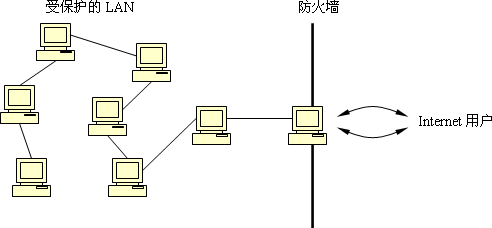
\includegraphics[scale=0.5]{network_firewall.png}
\caption{Firewall}
\label{network_firewall}
\end{figure}


防火墙会强制执行一个组织的访问控制策略(Access Control Policy),来执行接受和拒绝什么类型的网络通信。例如一个特定的组织可能只允许它的用户和外界以Email进行网络通信,拒绝其他任何通信方式,如站点访问等。另一个组织可能允许用户自由访问Internet,但不想让一般的Internet用户渗透到它的系统中或访问它的数据。组织的系统管理员将为他们的LAN设置防火墙,接受“可接受”类型的通信,拒绝其他类型的通信。实现这一点的方法有很多,最简单的一种是用端口号拒绝通信。例如,可建立防火墙,通过拒绝由端口23进入的所有通信,能够阻止LAN之外的用户创建对LAN之内机器的telnet连接。


更复杂的防火墙系统能维护有关流经它们的通信的状态的内部信息或存储数据本身,防火墙能够决定的通信状态越多,就越能保护它的用户。当然,这种安全是有代价的,有些防火墙会给网络通信带来明显的延迟。

不幸地是,很多微软的 windows 用户都意识不到其网络设置中常见的安全漏洞。下面是 Microsoft Windows 中常见的网络组件安装列表:

\begin{compactitem}
\item Microsoft 网络客户端
\item Microsoft 的文件和打印机网络共享
\item Internet 协议(TCP/IP )
\end{compactitem}

允许在 TCP/IP 上使用 NetBIOS,那么会面临一个安全问题:

\begin{compactitem}
\item 文件会被整个 Internet 共享
\item 用户的登录名、计算机名称以及工作组名称对其他人都是可见的
\end{compactitem}

而允许 TCP/IP 上的文件和打印机共享,也会面临安全问题:

\begin{compactitem}
\item 文件会被整个 Internet 共享
\end{compactitem}

没有连接任何网络的计算机也可能拥有危险的网络设置,这是由于一旦 Internet 被安装,网络设置就会发生改变。

上述的情况的解决方案是在网络连接属性中禁用 NetBIOS 协议和文件打印机共享,具体的操作方法会因不同的 windows 版本而略有不同。如果仍然需要在网络上共享打印机和文件,可以选择使用 NetBEUI 协议来代替 TCP/IP 协议。







\chapter{Network Address}

在通过计算机网络进行通信时,最终都是在与世界上某处的另一台计算机通信,因此Internet网络的地址必须精确到一台特定的机器,标识特定的机器以建立通信是一种相当复杂的机制。

主机名(Hostname)是Internet上的计算机的唯一标识,主机名通常是易读懂的单词,中间由点号分隔。例如:

\begin{lstlisting}[language=HTML]
matisse.csc.villanova.edu
condor.developcorp.com
theqiong.com
\end{lstlisting}


每个计算机必须有一个 IP 地址才能够连入因特网,每个 IP 包必须有一个地址才能够发送到另一台计算机。在处理Email地址和站点时,倾向于使用主机名,每个主机名对应一个IP地址,网络软件要把主机名翻译成对应的IP地址,便于计算机使用。

TCP/IP 使用 4 个数字来为计算机编址,每个计算机通常有一个唯一的 4 个十进制数的地址,中间由点号分隔,唯一的标识了Internet上的机器。例如:


\begin{lstlisting}[language=HTML]
205.39.145.18
193.133.20.4
\end{lstlisting}


整个Internet协议都是以32位(bit)的IP地址为基础的,也就是说TCP/IP 使用 32 个比特来编址,一个IP地址长为32位,IP地址中的每个数对应IP地址中的一个字节。

由于一个字节(8位)可以表示256种事物,所以IP地址中的数字的范围是0到255,即从00000000、00000001、00000010、00000011、00000100、00000101、00000110、00000111、00001000 ……直到 11111111,如下图所示:

\begin{figure}[!h]
\centering
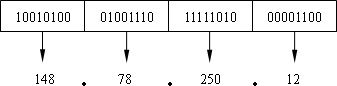
\includegraphics[scale=0.5]{network_ip_address.png}
\caption{IP地址}
\label{network_ip_address}
\end{figure}



虽然主机名和IP地址都是由点号分隔成几个部分,但是它们的每个部分之间不存在对应关系,整个主机名对应一个IP地址,而且IP地址一定有4个值,而主机名包含几部分是不确定的。

可以把IP地址分割成网络地址(Network Address),指定一个特定的网络和主机号,后者指定了网络中的一台特定机器。


如何分隔IP地址是由它表示的网络的类别决定的。不同大小的网络具有不同的网络类(A、B和C)。


A类网络把第一个字节作为网络地址,其他三个字节用作主机名。B类网络把前两个字节作为网络地址,后两个字节用作主机号,C类网络把前三个字节作为网络地址,最后一个字节用作主机号。

考虑一下采用这种寻址方法,每种网络的取值范围。A类网络比较少,但是每个网络中的主机较多。另一方面,C类网络很多,但每个网络中的主机很少。

大多数组织使用的是C类网络地址,A类和B类网络地址是为大型组织和ISP保留的。


\section{Domain Name}

主机名是由计算机名加域名构成的,例如,在主机名matisse.csc.villanova.edu中,matisse是计算机名,csc.villanova.edu是域名。

主机名中说明特定的组织或分组的部分叫做域名,域名由两个或多个部分组成,它们说明了计算机所属的组织或组织的一个子集。例如在这个例子中,matisse是Villanova大学的计算机系的一台计算机。

域名仅限于由特定组织控制的一组特定网络,而且不同组织中的计算机可以重名,因为从域名可以分辨出引用的是哪一台计算机。





域名中的最后一部分叫做顶级域名(Top-Level Domain,TLD),TLD声明了组织的类型或所属国家,下表列出了主要的顶级域名。

\begin{table}
\centering
\caption{主要的顶级域名}
\label{top_level_domain}
\begin{tabular}{|p{60pt}|p{60pt}|p{60pt}|p{60pt}|}
\hline
顶级域名		&用途		&	新顶级域名	& 用途\\
\hline
.com			&公司		& .biz			&商业\\
\hline
.net			&网络		&.info			&信息\\
\hline
.org			&非营利组织	&.pro			&专业\\
\hline
.edu			&教育部 		&.museum 		&博物馆\\
\hline
.int			&国际 		&.aero 			&航空业\\
\hline
.mil			&陆军 		&.coop			&合作团体\\
\hline
.gov			&政府 		&				&\\
\hline

\end{tabular}
\end{table}

每种域名用于一种特定类型的组织,例如.com用于商业组织,.edu用于大学和学院,美国以外的国家的组织采用国家代码作为顶级域名。下表列出了部分国家代码。

\begin{table}
\centering
\caption{部分国家代码}
\label{nation_code}
\begin{tabular}{|p{100pt}|p{100pt}|}
\hline
国家代码TLD	&国家\\
\hline
.au			&澳大利亚\\
\hline
.br			&巴西\\
\hline
.ca			&加拿大\\
\hline
.gr			&希腊\\
\hline
.in 			&印度\\
\hline
.ru 			&俄联邦\\
\hline
.uk 			&英国\\
\hline
\end{tabular}
\end{table}


最初,任何人或任何组织都可以注册自己的域名,只要这个名字还没被用到即可。

现在顶级域名(如.com和.edu)已经变得拥挤不堪了,已经为了缓解目前域名使用存在的问题,通过了新的顶级域名集合。

新的顶级域名注册制度使用新TLD的域名受到了限制,只有具有商标专用权的组织才能申请对应的域名。

域名注册的另一个来源是过期的域名。当注册了一个域名后,假设没有法律或商标方面的争议,那么只要付清费用(可以提前支付 10 年的费用),就可以自由地使用任意长的时间。




\section{Sub Domain Name}


大多数人们都没有意识到,但确实是每天都在使用着子域名。在Internet上可以见到很多子域名的例子:比如 store.apple.com 和 support.microsoft.com,最常见的 "www" 其实就是典型的子域名。

子域名可以在 DNS服务器上创建,并且不需要通过域名注册机构来进行注册。当然,在创建子域名之前,还是需要首先注册原始域名的,然后就可以请求网站主机提供商来创建子域名,也可以通过管理DNS服务器来创建。

某些提供商可能会为用户提供一个位于其域名之下的一个唯一的名称:www.theircompany.com/yourcompany/,但这并不是一个真实的域名,而是一个目录,而且应当尽量避免这样的情况。

这种 URL 的典型运用是通过 ISP 用于个人网站或免费网站,其实就是分享一个独立域名的方式,可为用户提供属于自己的地址。




\section{Domain Name System}

用于 TCP/IP 地址的名字被称为域名,域名系统(DNS,Domain Name System)主要用于把域名翻译成数字IP地址。

在DNS建立之前,斯坦福大学的一个研究小组负责维护一个文件主机表。每建立一个新主机名,斯坦福小组就把它添加到该表(每周两次),系统管理员会读取修改过的主机表,更新他们的域名服务器(把主机名翻译(解析)成IP地址的计算机)。

随着主机名数量的增长,只用一个表记录主机名已经不可行了,对于更新和分发信息来说,它不是一种实用的方法。1984年,网络工程师设计出了目前使用的复杂域名系统。


在全世界,数量庞大的 DNS 服务器被连入因特网,DNS已经从最初包括所有信息的单个文件发展成了把任务分配给几百万个域名服务器的分布式系统,其本身也演变成了一种分布式数据库,没有一个组织要负责更新主机名/IP映射。

DNS 服务器负责将域名翻译为 TCP/IP 地址,同时负责使用新的域名信息更新彼此的系统。当一个新的域名连同其 TCP/IP 地址一同注册后,全世界的 DNS 服务器都会对此信息进行更新。

现在,域名被称为是网站的唯一名称,当域名被注册后,就会被添加到大的域名注册商那里,连同与网站有关的信息——包括被保存在 DNS 服务器的 IP 信息,现在DNS服务器的功能包括负责向 Internet上的其他计算机通知有关你的域名和地址的信息。


在网络浏览器窗口或Email地址中指定了一个主机名时,浏览器或Email软件将给附近的域名服务器发送一个请求。如果这台服务器可以解析主机名,则进行解析,否则这台服务器将把这个请求转发给另一台域名服务器。如果第二台域名服务器也不能解析它,会继续转发这个请求,最终该请求到达一台能够解析它的服务器,或者因为解析时间太长而过期。



\chapter{WWW}

万维网的全名是World Wide Web,简称Web,与Internet相比,Web是个相对较新的概念,而且两者有着本质的不同。




从20世纪50年代开始,网络就用于连接计算机,这也是早期的Internet的雏形。虽然Internet已经用于通信多年了,但早期的通信几乎都是采用基于文本的Email和基本的文件交换实现的。



Web是与使用网络交换信息的软件结合在一起的分布式信息的基础设施,从而人们可以通过鼠标点击和图形界面操作,得到任何想要的资源。



WWW 是一张遍布全球的计算机网络,Web 中的所有计算机均可彼此相互通信,所有的计算机都使用被称为 HTTP 的通信标准。

Internet使通信成为了可能,而Web则使通信变得轻松、丰富和有趣。在Internet出现之后,直到20世纪90年代中期才出现了Web,从而使Internet普及到个人和家庭,也使Internet成为了商业的主要通信工具,自此以后,电子商务、电子支付、财务事项往来和小组管理变成了常见的在线活动,这也是Web对日常生活方式和商业模式的影响。

Web 信息存储于被称为网页(Web Page)的文档中,网页是存储于名为Web服务器的计算机中的文件。Unix 是首个(或最原始的)Web服务器操作系统,并以可靠性和稳定性而闻名。


读取网页的计算机可称为Web客户机,Web客户机通过名为Web浏览器的程序来查看页面。

网页中包括或引用各种数据,这些数据包括文本、图像、图形或程序。Web页还包含对其他Web页的链接(link),以便用户能够使用计算机鼠标在用户界面上跳转。

Web站点(Site)是一组相关的Web页,这组Web页通常是由个人或公司设计和控制的,Web站点的设计和实现技术多种多样。



在使用Web时,要“访问”一个Web站点,其实就是请求存储在远程Web服务器上的Web页,把它传输到本地计算机上以便浏览。

在Web服务器上,网页可作为 CGI 脚本来执行。CGI 脚本可在服务器上执行,来生成动态的交互性页面。大多数的 ISP 都会提供对 CGI 的某种程度的支持。并且许多都提供了使用 CGI 编写的预先安装的可运行的留言簿、页面计数器以及聊天/论坛解决方案。


所有的网页都含有供显示的指令,浏览器通过读取这些指令来显示页面,其中最常用的显示指令是 HTML 标签。只要客户机说明想要的信息,它们就会通过Web浏览器呈现在我们面前。



我们使用Web浏览器(Browser)在Web上通信,Web浏览器是处理Web页的请求并在它到达后将它显示出来的软件工具,例如Netscape Navigator、Internet Explorer、Mozilla Firefox、Apple Safari、Opera、Google Chrome等。对于网站开发人员来说,Web浏览器信息和统计数据的非常重要的。


浏览器可以通过一个请求 (request) 从Web服务器读取页面,其中请求是包含页面地址的标准 HTTP 请求,地址看上去类似这样:http://www.theqiong.com/index.html。


通过浏览器获取一个Web页的过程可以表示如下:

\begin{figure}[!h]
\centering
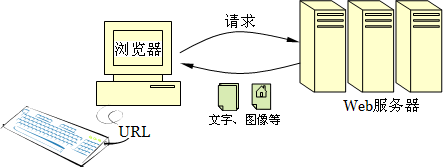
\includegraphics[scale=0.5]{network_browser.png}
\caption{通过浏览器获取一个Web页的过程}
\label{network_browser}
\end{figure}


被请求的Web页通常存储在另一台计算机上,用于响应Web请求的计算机就叫做Web服务器(Server)。Web页包含文本和其他独立的元素,比如图像。在请求Web页之后,所有与这个页面相关的元素都会被返回浏览器中。


在浏览器中,我们用Web地址说明我们想要的Web页,例如:www.villanova.com/academics.html

Web地址是统一资源地址(Uniform Resource Locator,URL)的核心部分,可以使用URL指定我们想要浏览的Web文档。URL唯一标识了存储在世界各处的Web页,而且URL的一部分是存储信息的计算机的主机名。



所有的 W3C 标准(自从1996年),包括 HTML、XHTML 和 XML 都定义了一个名为 Unicode (ISO 10646) 内部的内部字符集。

所有现代Web浏览器都在原生地使用此字符集,然而大多数在 internet 上传输的文档并没有使用这个 Unicode 字符集,因此Internet 客户(浏览器)与 Internet 服务器之间必须有一种在通信中一致使用字符集的方法。

对每个文档在用的字符集进行标记,对于提升网站的品质来说至关重要,推荐始终在 <head> 元素内 使用下面的的元元素:

\begin{lstlisting}[language=HTML]
<meta http-equiv="Content-Type" content="text/html;charset=utf-8" />
\end{lstlisting}

这里的charset是网页所使用的字符集,比如ISO-8859-1、UTF-8 或者 UTF-16。

类似 "04-03-02" 的日期格式在网页上可能被表示为2004年3月2日,或者2002年3月4日,亦或者2002年4月3日,因此国际标准化 (ISO) 为日期定义的国际标准格式是 "yyyy-mm-dd",yyyy 是年,mm 是月,dd 是日。


\section{Email}


POP(邮局协议)是一种用于发送和接收电子邮件的标准客户机/服务器协议。电子邮件会被接收并保存到internet 服务器上,直到用户通过某个客户段邮件程序(比如 Outlook 和 Foxmail)来收取信件。


IMAP 指的是 Internet 消息访问协议,这是另外一种用于发送和接收电子邮件的标准协议。

IMAP 在 POP 的基础上提供了一定的改进,即存储在 IMAP 服务器上的电子邮件可以由多台计算机处理,而无需在计算机间来回传输消息,而 POP 被设计为支持在一台单独的计算机上进行的邮件访问。


基于Web的电子邮件使用户通过Web浏览器就可以访问电子邮件。通过Web登陆到电子邮件帐户以后就可以发送和接收电子邮件了,能够从世界上的任何地方访问电子邮件是件很吸引人的事情。


\section{Search Engine}

Web搜索引擎是帮助用户找到其他站点的站点,比如Google和Yahoo!等。在搜索引擎中,用户通过输入单词或关键字(key word),说明你想要找的信息的类型,搜索引擎就会根据这些搜索相关信息,给用户提供一个有可能匹配检索要求的候选站点列表。

第一个因特网搜索工具叫做Archie,这是加拿大麦吉尔大学的计算机系学生在1990年开发的。Archie针对因特网上所有的匿名登录FTP站点设立了一个可供搜索和下载的数据库,这正是搜索引擎的雏形。

搜索引擎是通过检索具有上百万个站点的信息的数据库来生成候选站点列表的。好的搜索引擎会保持自己的数据库是最新的,而且具有匹配关键字和Web页内容的有效技术。有些搜索引擎只是以用户输入的关键字为依据,而有些则会尝试解释关键字的内涵,比如通过上下文匹配等。

大多数搜索引擎是通过用户输入的关键字与作为站点索引的一组关键字进行比较来确定搜索结果的。有些搜索引擎几乎把每个Web页上的每个单词都作为索引存入数据库的,只是除去“a”、“an”和“the”这样的常用单词。有些搜索引擎则只用Web页的部分内容作为索引,如文档的标题和副题等。有些索引技术区分大小写,有些则不区分。

关键字检索非常具有挑战性,因为自然语言(如英语)本身具有二义性,例如,术语hard cider(烈性苹果酒)、hard brick(坚硬的砖)、hard exam(很难的测验)和hard drive(磨损的道路)中的hard的意思都不同。如果提供了足够的关键字,搜索引擎能够正确地区分匹配站点的优先次序,但是在没有上下文的情况下,基本的关键字匹配是很有限的。

有些搜索引擎执行基于概念的搜索,即尝试判断所执行的搜索的上下文。如果它们运行的很好,返回的候选页会包含要检索的主题的相关内容,无论这个页面中的单词是否与查询中的关键词完全匹配。

执行基于概念的搜索的技术有几种,它们通常以复杂的语言理论为基础,这些技术的基本前提是分类,即对比相近的单词。例如,在医学领域中,心脏这个词可能与动脉、胆固醇和血这些词相近。

基于概念的搜索引擎比关键字检索复杂的多,而且现在基于概念的搜索技术还很不完善,这种技术在搜索引擎发展中很有潜力。



\section{IM}



即时消息(Instant Message)应用程序可能是目前最受欢迎的Web程序,它给了Web另一种交互方式。使用这些IM程序,可以实时地给朋友或工作伙伴发送消息,进行在线交流。如果发送者和接收者同时运行了即时消息程序,那么消息一到达就会立刻提醒或展示在用户面前,这样两个人就能够进行在线交流。现在领先的IM应用程序包括America Online(AOL)Instant Messenger(AIM)和Tencent QQ。

IM应用程序发展到现在,可以允许用户定制联系人列表,设置默认的答复,除了文本外,还可以发送标准的图形或订制的图形,IM模式已经成为了许多用户的标准通信方式,现在IM程序已经发展成了具有图像和视频等应用。

大多数IM应用程序使用专有的协议,规定发送信息的格式和结构,比如AIM的协议也是专有的,但并不限于AOL用户才能使用,这也促进了AOL的流行。

IM应用程序虽然方便,但却并不安全,通过各种IM协议发送的消息并没有加密,可能会被网络通途中的中间点截获,未加密的Email也同样不安全。

\chapter{W3C}

万维网联盟(World Wide Web Consortium,W3C)创立了 WWW 标准,W3C 的使命是通过发展规范、指导方针、软件以及工具,来尽展万维网潜能。

“web 蕴藏的梦想是一个可在其中通过分享信息而进行通信的公共信息空间。”

\begin{flushright}
——Tim Berners-Lee,万维网的发明人,W3C 的主任及创立者
\end{flushright}

万维网(World Wide Web)是作为欧洲核子研究组织的一个项目发展起来的,这那里 Tim Berners-Lee 开发出万维网的雏形。

W3C 在 1994 年被创建的目的是,为了完成麻省理工学院(MIT)与欧洲粒子物理研究所(CERN)之间的协同工作,并得到了美国国防部高级研究计划局(DARPA)和欧洲委员会(European Commission)的支持。现在,W3C是一个致力于“尽展万维网潜能”的国际性联盟。

\begin{compactitem}
\item W3C 指万维网联盟(World Wide Web Consortium)
\item W3C 被创建于 1994 年 10 月
\item W3C 由 Tim Berners-Lee 创立
\item W3C 由Web的发明人创立
\item W3C 以会员机构的形式进行组织
\item W3C 致力于对Web进行标准化
\item W3C 创建并维护了 WWW 标准
\item W3C 标准被称为 W3C 推荐标准(W3C Recommendations)
\end{compactitem}

W3C 致力于实现所有的用户都能够对Web加以利用(不论其文化教育背景、能力、财力以及其身体残疾),其最重要的工作是发展Web规范(称为推荐,Recommendations),这些规范描述了Web通信协议(比如 HTML 和 XML)和其他构建模块的“推荐标准”,最重要的 W3C 标准包括:

\begin{compactitem}
\item HTML
\item XHTML
\item CSS
\item XML
\item XSL
\item DOM
\end{compactitem}

每项 W3C 推荐的发展是通过由会员和受邀专家组成的工作组来完成的。工作组的经费来自公司和其他组织,并会创建一个工作草案,最后是一份提议推荐。一般来说,为了获得正式的批准,推荐都会被提交给 W3C 会员和主任。

W3C 同时与其他标准化组织协同工作,比如 Internet 工程工作小组(Internet Engineering Task Force)、无线应用协议(WAP)以及 Unicode 联盟(Unicode Consortium)。

目前,W3C由美国麻省理工学院计算机科学和人工智能实验室 (MIT CSAIL),总部位于法国的欧洲信息数学研究联盟 (ERCIM) 和日本的庆应大学(Keio University)联合运作,并且在世界范围内拥有分支办事处。

正因为 Web 是如此的重要(不论在其影响范围还是在投资方面),以至于不应由任何一家单独的组织来对它的未来进行控制,因此 W3C 扮演者一个会员组织的角色:

\begin{compactitem}
\item IBM
\item Microsoft
\item America Online
\item Apple
\item Adobe
\item Macromedia
\item Sun Microsystems
\item ...
\end{compactitem}

W3C 的会员包括了软件开发商、内容提供商、企业用户、通信公司、研究机构、研究实验室、标准化团体以及政府。

W3C 国际化活动的目标是,在 W3C 内部以及与其他组织一起,建议并调整任何技术、协定、指导方针和活动,使得在不同的语言、脚本和文化范畴内更易在全球范围内使用 W3C 技术。


W3C 中国办事处成立于 2006 年 4 月 1 日。现设址于北京航空航天大学(BUAA),由北京航空航天大学计算机学院计算机新技术研究所负责日常运营工作。

W3C中国办事处致力于促进国内外万维网标准领域信息沟通互动,为国内企业、高校、及科研机构参与国际信息技术标准化的研究、集成和推广提供更好的服务。

W3C 在中国的会员包括:

\begin{compactitem}
\item 北京航空航天大学
\item 北京工业大学
\item 中国电子技术标准化研究所
\item 广州中间件研究中心
\item 安徽中科大讯飞信息科技有限公司
\item 倍多科技
\item 太原理工大学
\item ISTIC 中国科学技术信息研究所
\item Uncover China
\item Monotype Imaging Inc.
\item Industrial Technology Research Institute (ITRI) Taiwan
\item 香港特别行政区政府科技资讯总编办公室 (OGCIO)
\end{compactitem}

2009 年 11 月 14 日,W3C 及其中国办事处与全国各地关注 W3C 的志愿者团体和个人相聚北京,共议 W3C 中国社区建设计划启动事宜。

\section{W3C Procedure}

W3C 的标准化程序分为 7 个不同的步骤。在 W3C 发布某个新标准的过程中,规范是通过下面的严格程序由一个简单的理念逐步确立为推荐标准的:

\begin{compactitem}
\item W3C 收到一份提交
\item 由 W3C 发布一份记录
\item 由 W3C 创建一个工作组
\item 由 W3C 发布一份工作草案
\item 由 W3C 发布一份候选的推荐
\item 由 W3C 发布一份被提议的推荐
\item 由 W3C 发布推荐
\end{compactitem}

\begin{compactenum}
\item W3C 提交 (W3C Submissions)

任何 W3C 的成员都可向联盟提交希望成为 Web 标准的某项建议(案)。大多数W3C推荐都发源于向联盟做出的某个提交。

如果某项提交在 W3C 的工作领域(或宪章)内,那么 W3C 将决定是否启动对该项提议的改进工作。

\item W3C 记录 (W3C Notes)

通常,一项对 W3C 的提交会成为一份记录。记录是对作为一份公共文档来提炼的一项提议的描述。

W3C 仅把记录用户讨论。记录的发布并不代表对其的认可。记录的内容是由提交此记录的会员来编辑的,而不是 W3C。记录可在任何时间被更新、替换或废弃。记录的发布也不表明 W3C 已启动与此记录相关的任何工作。

\item W3C 工作组 (W3C Working Groups)

当某项提交被 W3C 承认,一个工作组就会成立,其中包括会员和其他有兴趣的团体。

工作组通常会定义一个时间表,并发布有关被提议标准的工作草案。

\item W3C 工作草案 (W3C Working Drafts)

W3C 工作草案通常会被发布于 W3C 的网站上,连同对公共注解的邀请。

工作草案会说明进行中的工作,但不应被用作任何参考材料。其内容可在任何时间被更新、替换或废弃。

\item W3C 候选推荐 (W3C Candidate Recommendations)

某些规范会比其他规范更复杂,并可能需要来自会员和软件开发商的更多的经费、更多时间以及更多测试。有时,这些规范会作为候选的推荐来发布。

候选的推荐也是一种“正在进行的工作”,同样不应被用作参考材料。此文档可在任何时间被更新、替换或废弃。

\item W3C 提议推荐 (W3C Proposed Recommendations)

提议的推荐意味着工作组中工作的最后阶段。

提议推荐也是一种“正在进行的工作”。此文档可在任何时间被更新、替换或废弃。不过即使它不意味着 W3C 的任何官方的认可,在极多的情况下,提议的推荐无论在内容还是时间上都已接近于最后的推荐。

\item W3C 推荐 (W3C Recommendations)

W3C 推荐已经通过了 W3C 会员们的评审,并得到了 W3C 主任的正式批准。

W3C 推荐是一份稳定的文档,并可被用作参考材料。

\end{compactenum}





\section{W3C HTML}

HTML 2.0 是 1996 年由 Internet 工程工作小组的 HTML 工作组开发的。现在HTML 2.0 已经是过时的 HTML 版本。目前在市场上可以找到的浏览器都依赖于更新版本的 HTML。对于一位 WEB 开发者而言,没有任何必要需要 HTML 2.0 标准。

HTML 3.2 作为 W3C 标准发布于 1997 年 1 月 14 日。HTML 3.2 向 HTML 2.0 标准添加了被广泛运用的特性,诸如字体、表格、applets、围绕图像的文本流,上标和下标,其中被添加到 1997 年 HTML 3.2 标准的元素之一 - <font> 标签 - 为 HTML 内容和呈现的分离这个重要的任务带来了不必要的麻烦。

作为一项 W3C 推荐,HTML 4.0 被发布于 1997 年 12 月 18 日,HTML 4.0 最重要的特性是引入了样式表(CSS)。而仅仅进行了一些编辑修正的第二个版本发布于 1998 年 4 月 24 日。



作为一项 W3C 推荐,HTML 4.01 发布于 1999 年 12 月 24 日,HTML 4.01 是对 HTML 4.0 的一次较小的更新,对后者进行了修正和漏洞修复。

W3C 不会继续发展 HTML,未来 W3C 的工作会集中在 XHTML 上。作为一项 W3C 推荐,XHTML 1.0 发布于 2000 年 1 月 20 日。

XHTML 1.0 使用 XML 对 HTML 4.01 进行了重新地表示。



W3C 于 2008 年 1 月 22 日发布 HTML 5 工作草案。

HTML 5 中的新特性包括了嵌入音频、视频和图形的功能,客户端数据存储,以及交互式文档。

HTML 5 还包含了新的元素,比如:<nav>, <header>, <footer> 以及 <figure> 等等。

通过制定如何处理所有 HTML 元素以及如何从错误中恢复的精确规则,HTML 5 改进了互操作性,并减少了开发成本。

HTML 5 工作组包括:AOL, Apple, Google, IBM, Microsoft, Mozilla, Nokia, Opera, 以及数百个其他的供应商。

\begin{longtable}{|m{90pt}|m{90pt}|m{180pt}|}
%head
\multicolumn{3}{r}{}
\tabularnewline\hline
规范	& 草案/提议	&推荐
\endhead
%endhead

%firsthead
\caption{W3C HTML 规范和时间线}\\
\hline
规范	& 草案/提议	&推荐
\endfirsthead
%endhead

%foot
\multicolumn{3}{r}{}
\endfoot
%endfoot

%lastfoot
\endlastfoot
%endlastfoot
\hline
HTML 3.2	&&1997 年 1 月 14 日\\
\hline
HTML 4.0	&&1998 年 5 月 24 日\\
\hline
HTML 4.01	&&1999 年 12 月 24 日\\
\hline
HTML 5		&&2010 年 6 月 24 日(最新草案)\\
\hline

\end{longtable}




\section{W3C XHTML}

作为一项 W3C 推荐,XHTML 1.0 发布于 2000 年 1 月 26 日,XHTML 1.0 是使用 XML 对 HTML 4.01 进行的重新表示。

作为一项 W3C 推荐,XHTML 1.0 第二版发布于 2002 年 8 月 1 日。它不是一个新的版本,而是一次更新和漏洞修复。

XHTML 1.0 是自 1997 年以来对 HTML 的第一次主要的改变,同时也是在向更广泛的用户代理提供更丰富网页的道路上迈出的非常重要的一步,这些用户代理(代理)包括桌面电脑、移动设备和手机等等。

XHTML 是一项可从 HTML 4.01 平稳迁移的 XML 应用。W3C 把 HTML 4.01 重构为 XML 的第一个步骤,导致了 XHTML 1.0 的诞生。XHTML 1.0 依赖于 HTML 4.01 标签所提供的语义。

下一步是把 XHTML 模块化为更小的元素集合,使得 XHTML 和其他标记语言(比如矢量图形和多媒体)的结合更加容易。

同时,XHTML 的模块化还可以减少开发费用,改善与其它应用程序(比如数据库)的协同,更易与不同的用户代理(浏览器)进行通信,以及 HTML 和不同 XML 标准之间更纯净的整合。


XHTML 1.1 是一门严格的语言,且XHTML 1.1 不能向后兼容 HTML 4,小型设备(比如移动电话)也无法支持 XHTML 的全部功能。XHTML 1.1 将规范划分为具备有限功能的模型,小型浏览器只能通过支持选定的模型来减低其复杂性(不过一旦选定某个模型,就必须支持其全部特性)。

XHTML Basic 是 XHTML 1.1 的小型子集,它仅包含基本的 XHTML 特性,比如文本结构、图像、基本的标单以及基本的表格。它是为小型浏览器设计的(比如在手持设备中)。

正是由于 XHTML 中对 W3C 文档对象模型级别 2 的支持,事件处理器就可以依附在 XHTML 元素上,这样父元素就可以在子元素之前或之后来处理事件。

XHTML-Print 是 XHTML 1.1 (模块化的 XHTML) 的一部分,它被设计用于移动设备和廉价的打印机,这些设备通常可在没有打印缓存和为设备定制的打印驱动的情况下,将一张页面从头到尾打印出来。

XForms 是 HTML 表单的继任者,提供一种更完善且独立于呈现的 Web交 互事务处理方式。通过 XHTML 表单,用户可以访问某张页面,向页面添加信息,然后向Web服务器提交页面。

XForms被设计为与 XHTML 进行整合,我们期望未来的电子商务应用程序会需要需要 XForms。

XHTML 2.0 是下一代的标记语言。其功能性预计和 XHTML 1.1 很相似,但是可能被变更来遵守 XML 标准的要求,比如 XML Linking 和 XML Schema。

XHTML 1.0 的模块化是通过使用 XML DTD (Document Type Definition) 来实现的,而XHTML 2.0 的模块化是通过使用 XML Schemas 来实现的。

XLink 是在 XML 文档中创建超链接的一门语言。XLink 与 HTML 链接很相似 - 但是更加强有力地支持简单链接(比如 HTML)和扩展链接(用于把多项资源链接到一起)。

HLink 是对 XLink 的扩展,HLink 增加了一项能力,可规定在 XHTML 中元素哪项元素可表示超链接,并规定如何对超链接进行遍历。

\begin{longtable}{|p{180pt}|p{90pt}|p{90pt}|}
%head
\multicolumn{3}{r}{}
\tabularnewline\hline
规范	& 草案/提议	&推荐
\endhead
%endhead

%firsthead
\caption{W3C XHTML 规范和时间线}\\
\hline
规范	& 草案/提议	&推荐
\endfirsthead
%endhead

%foot
\multicolumn{3}{r}{}
\endfoot
%endfoot

%lastfoot
\endlastfoot
%endlastfoot
\hline
XHTML 1.0	 				&&2000 年 1 月 26 日\\
\hline
XHTML 1.0 修订版	 		&&2002 年 8 月 1 日\\
\hline
XHTML 1.1	 				&&2001 年 5 月 31 日\\
\hline
XHTML Modules	 			&&2001 年 4 月 10 日\\
\hline
XHTML Modules 1.1			&&2008 年 10 月 8 日\\
\hline
XHTML Basic	 			&&2000 年 12 月 19 日\\
\hline
XHTML Basic 1.1			&&2008 年 7 月 29 日\\
\hline
XHTML Events	 			&&2003 年 10 月 14 日\\
\hline
XHTML Print	 			&&2006 年 9 月 20 日\\
\hline
XHTML Media Types (SE)	&2009 年 1 月 16 日	 &\\
\hline
XHTML 2.0					&2006 年 7 月 26 日	 &\\
\hline
XForms 1.0	 				&&2003 年 10 月 14 日\\
\hline
XForms 1.0 (Third Edition)	&&2007 年 10 月 29 日\\
\hline
XForms 1.1					&2009 年 10 月 20 日	 &\\
\hline
XLink	 					&&2001 年 6 月 27 日\\
\hline
HLink						&2002 年 9 月 13 日	 &\\
\hline
\end{longtable}

\section{W3C XML}

XML 被设计用来描述、存储、传送及交换数据。


作为一项 W3C 推荐,XML 1.0 发布于 1998 年 2 月 10 日。

作为一项 W3C 推荐,XML 1.0 (SE) 发布于 2000 年 10 月 6 日。第二版仅仅是在合并第一版的勘误表的基础上进行的修正(漏洞修复),随后的第三版也仅仅是在合并第一版和第二版的勘误表的基础上进行的修正(漏洞修复)。

作为一份工作草案,XML 1.1 发布于2001 年 12 月 13 日,并作为一项候选推荐发布于2002年10月15日。XML 1.1 允许在名称中使用几乎所有的 Unicode 字符。

\begin{compactitem}
\item XML 命名空间(Namespaces)可规定一种方法,通过与 URI 引用相关联的方式,来定义在 XML 中使用的元素和属性名称。
\item XML Linking 语言 (XLink),允许您向XML文档中插入链接。
\item XML Pointer 语言 (XPointer),允许将地址链接到 XML 文档的具体部分。
\item XML Base 是一种用于对外部 XML 资源进行默认引用的标准。(与 HTML 中的 <base> 类似)。
\item XInclude 是一种使用元素、属性以及 URI 引用来合并 XML 文档的机制。
\end{compactitem}

\begin{longtable}{|p{180pt}|p{90pt}|p{90pt}|}
%head
\multicolumn{3}{r}{}
\tabularnewline\hline
规范	& 草案/提议	&推荐
\endhead
%endhead

%firsthead
\caption{W3C XML 规范和时间线}\\
\hline
规范	& 草案/提议	&推荐
\endfirsthead
%endhead

%foot
\multicolumn{3}{r}{}
\endfoot
%endfoot

%lastfoot
\endlastfoot
%endlastfoot
\hline
XML 1.0	 				&&1998 年 2 月 10 日\\
\hline
XML 1.0 (2.Ed)	 			&&2000 年 10 月 6 日\\
\hline
XML 1.0 (3.Ed)	 			&&2004 年 2 月 4 日\\
\hline
XML 1.1	 				&&2004 月 2 月 4 日\\
\hline
XML 1.1 (2.Ed)	 			&&2006 年 8 月 16 日\\
\hline
XML 1.0 Namespaces		&&	 	1999 年 1 月 14 日\\
\hline
XML 1.0 Namespaces SE 	&&	 	2004 年 3 月 4 日\\
\hline
XML 1.1 Namespaces		&& 	2004 年 3 月 4 日\\
\hline
XML 1.1 Namespaces SE 	&&	 	2006 年 8 月 16 日\\
\hline
XML Infoset	 				&&2001 年 10 月 24 日\\
\hline
XML Infoset (2.Ed)	 		&&2004 年 2 月 4 日\\
\hline
XML Base	 				&&2001 年 6 月 27 日\\
\hline
XLink 1.0	 				&&2001 年 6 月 27 日\\
\hline
XPointer Framework		&&	2003 年 3 月 25 日\\
\hline
XPointer element() scheme	&& 	2003 年 3 月 25 日\\
\hline
XPointer xmlns() scheme	&& 	2003 年 3 月 25 日\\
\hline
XInclude 1.0	 			&&2004 年 12 月 20 日\\
\hline
XInclude 1.0 SE	 			&&2006 年 11 月 15 日\\
\hline
XML Processing Model		&2004 年 4 月 5 日	 &\\
\hline
XMLHttpRequest Object		&2010 年 8 月 3 日	 &\\
\hline
\end{longtable}


\section{W3C CSS}

CSS 是一种向网页添加样式的机制,用于描述文档如何被显示、发音或打印。

作为一项 W3C 推荐,CSS1 发布于 1996 年 12 月 17 日。1999 年 1 月 11 日,此推荐被重新修订。

作为一项 W3C 推荐,CSS2 发布于 1999 年 1 月 11 日。CSS2 添加了对媒介(打印机和听觉设备)和可下载字体的支持。

CSS3 计划将 CSS 划分为更小的模块。

\begin{longtable}{|p{180pt}|p{90pt}|p{90pt}|}
%head
\multicolumn{3}{r}{}
\tabularnewline\hline
规范	& 草案/提议	&推荐
\endhead
%endhead

%firsthead
\caption{W3C CSS 规范和时间线}\\
\hline
规范	& 草案/提议	&推荐
\endfirsthead
%endhead

%foot
\multicolumn{3}{r}{}
\endfoot
%endfoot

%lastfoot
\endlastfoot
%endlastfoot
\hline
CSS 1	 			&&1996 年 12 月 17 日\\
\hline
CSS 1 (Revised)	 	&&1999 年 1 月 11 日\\
\hline
CSS 2	 			&&1998 年 5 月 12 日\\
\hline
CSS 2.1				&2007 年 7 月 19 日	 &\\
\hline
CSS 2 Mobile		&2007 年 10 月 19 日	 &\\
\hline
CSS 2 TV			&2003 年 5 月 14 日	 &\\
\hline
CSS 2 Print			&2006 年 10 月 13 日	 &\\
\hline
CSS 3				&2001 年 5 月 23 日	 &\\
\hline
CSS 3 Namespace	&2006 年 8 月 28 日	 &\\
\hline
CSS 3 User Interface&	2004 年 5 月 11 日	 &\\
\hline
CSS 3 Selectors		&2005 年 12 月 15 日	 &\\
\hline
CSS 3 Fonts		&2002 年 8 月 2 日	 &\\
\hline
CSS 3 Web Fonts	&2002 年 8 月 2 日	 &\\
\hline
CSS 3 Colors		&2003 年 5 月 14 日	 &\\
\hline
CSS 3 TV			&2003 年 5 月 14 日	 &\\
\hline
CSS 3 Backgrounds and borders	&2005 年 2 月 16 日	 &\\
\hline
CSS 3 Text			&2007 年 3 月 6 日	 &\\
\hline
CSS 3 Lists			&2002 年 11 月 7 日	 &\\
\hline
CSS 3 Line			&2002 年 5 月 15 日	 &\\
\hline
CSS 3 Box model	&2007 年 8 月 9 日	 &\\
\hline
CSS 3 Multi column	&2007 年 6 月 6 日	 &\\
\hline
CSS 3 Ruby			&2003 年 5 月 14 日	 &\\
\hline
CSS 3 Border		&2005 年 3 月 16 日	 &\\
\hline
CSS 3 Speech		&2004 年 12 月 16 日	 &\\
\hline
CSS 3 Paged Media (PM)	 &2006 年 10 月 10 日	 &\\
\hline
CSS 3 Generated PM	&2007 年 5 月 4 日	 &\\
\hline
CSS 3 Print			&2006 年 10 月 13 日	 &\\
\hline
CSS 3 Values		&2006 年 9 月 19 日	 &\\
\hline
CSS 3 Cascade		&2005 年 12 月 15 日	 &\\
\hline
CSS 3 Template Layout	&2009 年 4 月 2 日	 &\\
\hline
CSS 3 Media Queries	&2009 年 9 月 15 日	 &\\
\hline


\end{longtable}


\section{W3C XSL}


XSL 语言包括三部分:XSLT、XPath 以及 XSL 格式化对象。


作为一项 W3C 推荐标准,XSL 1.0 作为一门表达样式表的语言被发布于 2001 年 10 月 15 日。它由三部分组成:XSLT、XPath 以及 XSL 格式化对象。

XSLT 1.0于 1 999年11月16日成为 W3C 推荐标准。XSLT 是一门用于把 XML 文档转换为其他 XML 文档的语言。


XSLT 2.0于 2007 年 1 月 23 日成为 W3C 推荐标准。


XSL-FO (XSL 格式化对象)是一个用于规定格式化语义的词汇表。

格式化指的是把XSL转换的结果转变为适合阅读器或收听器的过程。虽然不存在针对 XSL 格式化对象的独立 W3C 文档,但是还是可以在 XSL 1.0 推荐标准中找到相关的描述。

\begin{longtable}{|p{180pt}|p{90pt}|p{90pt}|}
%head
\multicolumn{3}{r}{}
\tabularnewline\hline
规范	& 草案/提议	&推荐
\endhead
%endhead

%firsthead
\caption{W3C XSL 规范和时间线}\\
\hline
规范	& 草案/提议	&推荐
\endfirsthead
%endhead

%foot
\multicolumn{3}{r}{}
\endfoot
%endfoot

%lastfoot
\endlastfoot
%endlastfoot
\hline
XSL 1.0 (XSL-FO)	 	&&2001 年 10 月 15 日\\
\hline
XSL 1.1	 				&&2006 年 12 月 5 日\\
\hline
XSLT 1.0	 			&&1999 年 11 月 16 日\\
\hline
XSLT 1.1				&2001 年 8 月 24 日	&\\
\hline 
XSLT 2.0 Requirements	&2001 年 2 月 14 日	&\\
\hline 
XSLT 2.0	 			&&2007 年 1 月 23 日\\
\hline

\end{longtable}


\section{W3C XML Schema}

XML Schema 是基于 XML 的 DTD 替代物,XML Schema 对应用程序、文档结构、属性和数据类型有着更良好的支持。




XML 1.0 支持可定义文档结构的 DTD,未来的 XML 版本有赖于 XML Schema 来定义 XML 文档的类型。


\begin{compactitem}
\item XML Schema 的结构(XML Schema Structure)规定了 XML Schema 的定义语言。
\item XML Schema 的数据类型为 XML 规定了可扩展的数据类型。
\end{compactitem}


\begin{longtable}{|p{180pt}|p{90pt}|p{90pt}|}
%head
\multicolumn{3}{r}{}
\tabularnewline\hline
规范	& 草案/提议	&推荐
\endhead
%endhead

%firsthead
\caption{W3C XML Schema 规范和时间线}\\
\hline
规范	& 草案/提议	&推荐
\endfirsthead
%endhead

%foot
\multicolumn{3}{r}{}
\endfoot
%endfoot

%lastfoot
\endlastfoot
%endlastfoot
\hline
XML Schema	 			&&2001 年 5 月 2 日\\
\hline
XML Schema Structures	 	&&2001 年 5 月 2 日\\
\hline
XML Schema Datatypes	 	&&2001 年 5 月 2 日\\
\hline
XML Schema (2.Ed)	 		&&2004 年 10 月 28 日\\
\hline
XML Schema Structures (2.Ed)&&	 	2004 年 10 月 28 日\\
\hline
XML Schema Datatypes (2.Ed)&&	 	2004 年 10 月 28 日\\
\hline
XML Schema Component Designators&	2008 年 11 月 17 日&\\
\hline	 
XML Schema 1.1: Structures	 	&&2009 年 4 月 30 日\\
\hline
XML Schema 1.1: Datatypes	 	&&2009 年 4 月 30 日\\
\hline

\end{longtable}


\section{W3C XPath}



XPath 是一门用于选取 XML 文档的部件的语言,它被设计为供 XSLT、XQuery 以及 XPointer 使用。


XPath 1.0 于 1999 年 11 月 16 日成为 W3C 推荐标准。


XPath 2.0 于 2007 年 1 月 23 日成为 W3C 推荐标准,它是一门由 XPath 1.0 和 XQuery 衍生而来的语言。

XPath 2.0 和 XQuery 1.0 的产生是同源的,它们拥有不少相同的语法,而且不少文本也是一致的。




\begin{longtable}{|p{180pt}|p{90pt}|p{90pt}|}
%head
\multicolumn{3}{r}{}
\tabularnewline\hline
规范	& 草案/提议	&推荐
\endhead
%endhead

%firsthead
\caption{W3C XPath 规范和时间线}\\
\hline
规范	& 草案/提议	&推荐
\endfirsthead
%endhead

%foot
\multicolumn{3}{r}{}
\endfoot
%endfoot

%lastfoot
\endlastfoot
%endlastfoot
\hline
XPath 1.0	 			&&1999 年 11 月 16 日\\
\hline
XPath 2.0 Requirements	&2005 年 6 月 3 日	 &\\
\hline
XPath 2.0 Language	 	&&2007 年 1 月 23 日\\
\hline
XPath 2.0 Functions	 	&&2007 年 1 月 23 日\\
\hline
XPath 2.0 Data Model	&& 	2007 年 1 月 23 日\\
\hline
XPath 2.0 Semantics	&& 	2007 年 1 月 23 日\\
\hline
XPointer				&2002 年 8 月 16 日	 &\\
\hline
\end{longtable}


\section{W3C XQuery}

XQuery 是一门用于从 XML 文档中提取数据的语言,它是支持从 XML 文档提取数据的查询工具。

\begin{longtable}{|p{180pt}|p{90pt}|p{90pt}|}
%head
\multicolumn{3}{r}{}
\tabularnewline\hline
规范	& 草案/提议	&推荐
\endhead
%endhead

%firsthead
\caption{W3C XQuery 规范和时间线}\\
\hline
规范	& 草案/提议	&推荐
\endfirsthead
%endhead

%foot
\multicolumn{3}{r}{}
\endfoot
%endfoot

%lastfoot
\endlastfoot
%endlastfoot
\hline
XQuery Requirements	&2007 年 3 月 23 日	 &\\
\hline
XQuery Use Cases		&2007 年 3 月 23 日	 &\\
\hline
XQuery 1.0	 			&&2007 年 1 月 23 日\\
\hline
XQuery 1.0 Functions	&& 	2007 年 1 月 23 日\\
\hline
XQuery 1.0 Data Model	&& 	2007 年 1 月 23 日\\
\hline
XQuery 1.0 Semantics	&& 	2007 年 1 月 23 日\\
\hline
XQueryX	 			&&2007 年 1 月 23 日\\
\hline
XQuery 1.1 Requirements&	2007 年 3 月 23 日	 &\\
\hline
XQuery 1.1 Use Cases	&2008 年 12 月 3 日	 &\\
\hline
XQuery 1.1				&2008 年 12 月 3 日	 &\\
\hline
\end{longtable}




\section{W3C DOM}


文档对象模型 (DOM) 是一个平台,一个中立于语言的应用程序编程接口 (API),允许程序访问并更改文档的内容、结构和样式。


DOM 级别 0 不是 W3C 规范。而仅仅是对在 Netscape Navigator 3.0 和 Microsoft Internet Explorer 3.0 中的等价功能性的一种定义。W3C 的 DOM 级别 1 就是建立于此功能性之上。

DOM 发展过程中的关键角色有:ArborText、IBM、Inso EPS、JavaSoft、Microsoft、Netscape、Novell、the Object Management Group、SoftQuad、Sun Microsystems 以及 Texcel。



DOM 级别 1 于 1998 年 10 月 1 日成为 W3C 推荐标准,第二版的工作草案在 2000 年 9 月 29 日。

DOM 级别 1 专注于 HTML 和 XML 文档模型。它含有文档导航和处理功能。

DOM 级别 2 对 DOM 级别 1 添加了样式表对象模型,并定义了操作附于文档之上的样式信息的功能性。DOM 级别 2 同时还定义了一个事件模型,并提供了对 XML 命名空间的支持。

作为一项 W3C 推荐标准,DOM 级别 2 规范发布于 2000 年 11 月 13 日。

\begin{compactitem}
\item DOM Level 2 核心

DOM Level 2 核心 规定了访问和更改文档内容及结构的一个 API,此 API 同时包含用于 XML 的接口。

\item DOM Level 2 HTML

DOM Level 2 HTML 规定了操作 HTML 文档结构和内容的 API。(这部分规范仍然是工作草案)

\item DOM Level 2 Views

DOM Level 2 规定了对文档视图进行访问和更改的 API。视图是与原文档相关联的表现形式或某种备用的表现形式。

\item DOM Level 2 Style

DOM Level 2 Style 规定了动态访问及更改内容样式表的 API。

\item DOM Level 2 Events

DOM Level 2 Events 规定了访问文档事件的 API。

\item DOM Level 2 Traversal-Range

DOM Level 2 Traversal-Range 规定了动态遍历和识别文档中内容范围的 API。

\end{compactitem}


DOM Level 3 规定了内容模型 (DTD 和 Schemas) 和文档验证。同时规定了文档加载和保存、文档查看、文档格式化和关键事件。DOM Level 3 建立于 DOM Core Level 2 之上。

DOM Requirements 文档已经为 Level 3 requirements 进行了更新,并于 2000 年 4 月 12 日发布为工作草案。


下面的 DOM Level 3 工作草案发布于 2000 年 9 月 1 日:

\begin{compactitem}
\item DOM Level 3 Core

DOM Level 3 Core 规定了访问和更改文档内容、结构及样式的一个 API。

\item DOM Level 3 Events

通过增加新的接口和新的事件集,DOM Level 3 Events API 对 Level 2 Event API 的功能进行了扩展。

\item DOM Level 3 Load and Save

DOM Level 3 Content Model 规定了用于内容加载和保存、内容模型 (DTD and Schemas) 和文档验证支持的 API。

\item DOM Level 3 Views and Formatting

DOM Level 3 Views 规定了对文档视图进行访问和更改的 API。视图是与原文档相关联的表现形式或某种备用的表现形式。

\end{compactitem}

\begin{longtable}{|p{180pt}|p{90pt}|p{90pt}|}
%head
\multicolumn{3}{r}{}
\tabularnewline\hline
规范	& 草案/提议	&推荐
\endhead
%endhead

%firsthead
\caption{W3C DOM 规范和时间线}\\
\hline
规范	& 草案/提议	&推荐
\endfirsthead
%endhead

%foot
\multicolumn{3}{r}{}
\endfoot
%endfoot

%lastfoot
\endlastfoot
%endlastfoot
\hline
DOM Level 1	 		&&1998 年 10 月 1 日\\
\hline
DOM Level 1 (SE)		&2000 年 9 月 29 日	 &\\
\hline
DOM Level 2 Core	 	&&2000 年 11 月 13 日\\
\hline
DOM Level 2 HTML	 	&&2003 年 1 月 9 日\\
\hline
DOM Level 2 Views	 	&&2000 年 11 月 13 日\\
\hline
DOM Level 2 Style	 	&&2000 年 11 月 13 日\\
\hline
DOM Level 2 Events	 	&&2000 年 11 月 13 日\\
\hline
DOM Level 2 Traversal-Range&&	 	2000 年 11 月 13 日\\
\hline
DOM Level 3 Requirements	&2004 年 2 月 26 日	 &\\
\hline
DOM Level 3 Core	 		&&2004 年 4 月 7 日\\
\hline
DOM Level 3 Events			&2007 年 12 月 21 日	 &\\
\hline
DOM Level 3 Load and Save	&& 	2004 年 4 月 7 日\\
\hline
DOM Level 3 Validation	 	&&2004 年 1 月 27 日\\
\hline
DOM Level 3 XPath			&2004 年 2 月 26 日	 &\\
\hline
DOM Level 3 Views			&2004 年 2 月 26 日	 &\\
\hline
\end{longtable}



\section{W3C SOAP}

SOAP (Simple Object Access Protocol) 是一种中立于平台和语言的轻量级通信协议,使得程序可以通过标准的因特网 HTTP 进行通信。

Web Services 与应用程序到应用程序的通信有关,而SOAP就是基于 XML 的 Web Services 间的通信协议。


在 2000 年 5 月,SOAP 1.1 曾在一份记录中被建议到 W3C(由开发商:IBM,Lotus, Microsoft 以及 Userland),作为用于在分布式环境中交换信息的一种协议。

W3C SOAP 1.1 文档仅仅是一份用于讨论的记录(NOTE),此记录的发布不代表 W3C 对其任何程度的认可。

W3C 的 XML Protocol 工作组目前正工作于 SOAP 1.2,第一份工作草案发布于 2001 年 12 月 17 日。

SOAP 1.2 于 2003 年 6 月 24 日被发布为 W3C 推荐标准。


\begin{longtable}{|p{180pt}|p{90pt}|p{90pt}|}
%head
\multicolumn{3}{r}{}
\tabularnewline\hline
规范	& 草案/提议	&推荐
\endhead
%endhead

%firsthead
\caption{W3C SOAP 规范和时间线}\\
\hline
规范	& 草案/提议	&推荐
\endfirsthead
%endhead

%foot
\multicolumn{3}{r}{}
\endfoot
%endfoot

%lastfoot
\endlastfoot
%endlastfoot
\hline
SOAP 1.2 Primer	 		&&2003 年 6 月 24 日\\
\hline
SOAP 1.2 Primer SE	 		&&2007 年 4 月 27 日\\
\hline
SOAP 1.2 Messaging	 	&&2003 年 6 月 24 日\\
\hline
SOAP 1.2 Messaging SE	 	&&2007 年 4 月 27 日\\
\hline
SOAP 1.2 Adjuncts	 		&&2003 年 6 月 24 日\\
\hline
SOAP 1.2 Adjuncts SE	 	&&2007 年 4 月 27 日\\
\hline
SOAP 1.2 Test Collection	&& 	2003 年 6 月 24 日\\
\hline
SOAP 1.2 Test Collection SE	&& 	2007 年 4 月 27 日\\
\hline
SOAP 1.2 Attachments		&2004 年 6 月 8 日	 &\\
\hline
SOAP 1.2 Email Bindings	&2002 年 7 月 3 日	 &\\
\hline
SOAP 1.2 Normalization		&2003 年 10 月 8 日	 &\\
\hline
SOAP 1.2 Serialization		&2004 年 6 月 8 日	 &\\
\hline
Web Services Addressing 1.0 - Core	 	&&2006 年 5 月 9 日\\
\hline
Web Services Addressing 1.0 - SOAP	&& 	2006 年 5 月 9 日\\
\hline
\end{longtable}


\section{W3C WSDL}



前面提到,Web Services 与应用程序到应用程序的通信有关,而WSDL(Web Services Description Language)是一门基于 XML 的 Web Services 描述语言,确切地说,WSDL 是一种用于描述 Web Services 的 XML 格式。

作为一种可描述 Web Services 的 XML 格式,WSDL 1.1 于 2001 年 3 月曾在一份记录中被建议到 W3C(由Ariba、IBM 以及 Microsoft)。此记录还描述了如何结合 SOAP 1.1、HTTP GET/POST 以及 MIME 来使用 WSDL。

W3C WSDL 1.1 仅仅是用于讨论的记录(NOTE)。此记录的发布不代表 W3C 对其任何程度的认可。

关于WSDL 1.2的第一份工作草案发布于 2001 年 12月 17 日,最新的工作草案发布于 2003 年 6月 11 日。

W3C 的 XML Protocol 工作组目前正在工作于 WSDL 2.0。


\begin{longtable}{|p{180pt}|p{90pt}|p{90pt}|}
%head
\multicolumn{3}{r}{}
\tabularnewline\hline
规范	& 草案/提议	&推荐
\endhead
%endhead

%firsthead
\caption{W3C WSDL 规范和时间线}\\
\hline
规范	& 草案/提议	&推荐
\endfirsthead
%endhead

%foot
\multicolumn{3}{r}{}
\endfoot
%endfoot

%lastfoot
\endlastfoot
%endlastfoot
\hline
WSDL 1.1 Note				&2001 年 3 月 15 日	 &\\
\hline
WSDL Usage Scenarios		&2002 年 6 月 4 日	 &\\
\hline
WSDL Requirements			&2002 年 10 月 28 日	 &\\
\hline
WSDL Architecture			&2004 年 2 月 11 日	 &\\
\hline
WSDL Glossary				&2004 年 2 月 11 日	 &\\
\hline
WSDL Usage Scenarios		&2004 年 2 月 11 日	 &\\
\hline
WSDL 1.2 Core Language	&	2003 年 6 月 11 日	 &\\
\hline
WSDL 1.2 Message Patterns&	2003 年 6 月 11 日	 &\\
\hline
WSDL 1.2 Bindings			&2003 年 6 月 11 日	 &\\
\hline
WSDL 2.0 Primer	 		&&2007 年 6 月 26 日\\
\hline
WSDL 2.0 Core Language	&& 	2007 年 6 月 26 日\\
\hline
WSDL 2.0 Adjuncts	 		&&2007 年 6 月 26 日\\
\hline
WSDL 2.0 SOAP 1.1 Binding	&& 	2007 年 6 月 26 日\\
\hline
WSDL 2.0 RDF Mapping	 	&&2007 年 6 月 26 日\\
\hline
WS Addressing Core	 	&&2006 年 5 月 9 日\\
\hline
WS Addressing SOAP Binding&&	 	2006 年 5 月 9 日\\
\hline
Web Architecture	 	&&2004 年 12 月 15 日\\
\hline
\end{longtable}


\section{W3C RDF 和 OWL}



语义网是为资产管理、企业整合及网络数据的共享和重用提供的一个框架,为企业、应用程序、公司、团体和个人间的数据共享提供了一个独立于平台和软件的框架。


RDF 和 OWL是语义网的关键技术,它们分别阐述了结构性描述和以万维网为基础的本体论。


RDF(Resource Description Framework,资源描述框架)是一门向万维网表达信息的语言,可用于描述 web 资源,比如标题、作者以及版本信息、内容描述、可用时间表等等。

OWL(Web 本体语言) 是用于定义本体的语言,OWL 被设计为用于对信息进行处理(而不是现实信息)。

本体可以描述知识的领域,可供人类或软件用来分享有关对象的信息,这些对象可以是汽车、房屋、机器、书籍、产品、金融交易等等。

SPARQL(针对 RDF 的查询语言)是用于 RDF 数据的标准查询语言,可向开发者提供编写跨越 WEB 上广域 RDF 信息查询程序的途径。

\begin{longtable}{|p{180pt}|p{90pt}|p{90pt}|}
%head
\multicolumn{3}{r}{}
\tabularnewline\hline
规范	& 草案/提议	&推荐
\endhead
%endhead

%firsthead
\caption{W3C RDF 和 OWL规范和时间线}\\
\hline
规范	& 草案/提议	&推荐
\endfirsthead
%endhead

%foot
\multicolumn{3}{r}{}
\endfoot
%endfoot

%lastfoot
\endlastfoot
%endlastfoot
\hline
RDF Primer	 		&&2004 年 2 月 10 日\\
\hline
RDF Test Cases	 	&&2004 年 2 月 10 日\\
\hline
RDF Concept	 	&&2004 年 2 月 10 日\\
\hline
RDF Semantics	 	&&2004 年 2 月 10 日\\
\hline
RDF Schema	 		&&2004 年 2 月 10 日\\
\hline
RDF Syntax	 		&&2004 年 2 月 10 日\\
\hline
OWL Overview	 	&&2004 年 2 月 10 日\\
\hline
OWL Guide	 		&&2004 年 2 月 10 日\\
\hline
OWL Reference	 	&&2004 年 2 月 10 日\\
\hline
OWL Syntax	 	&&2004 年 2 月 10 日\\
\hline
OWL Test Cases	&& 	2004 年 2 月 10 日\\
\hline
OWL Use Cases	 	&&2004 年 2 月 10 日\\
\hline
Parsing OWL in RDF	&2004 年 1 月 21 日	&\\
\hline 
SPARQL Requirements&	2005 年 3 月 25 日&\\
\hline	 
SPARQL Language	 &&	2008 年 1 月 15 日\\
\hline

\end{longtable}

\section{W3C SMIL}



SMIL (Synchronized Multimedia Integration Language)是一门基于 XML 的类 HTML 语言,它被设计为用来启用 web 上的多媒体呈现。

1998 年 6 月 15 日,SMIL 1.0 成为 W3C 推荐标准,SMIL呈现可由音频、视频、图像、文本以及其他媒介类型组成。

HTML+TIME 指的是对 HTML 的定时多媒体交互扩展(Timed Interactive Multimedia Extensions for HTML)。它的作用是向 HTML 添加 SMIL 1.0 的定时和同步支持。

1998 年 9 月 18 日,作为一项向 HTML 增加了 SMIL 1.0 定时和同步的提议,HTML+TIME 被以下单位提交到 W3C :Microsoft、Macromedia、Compaq/Digital 以及 Digital Renaissance。

2000 年 2 月 25 日,HTML+TIME 以重新命名的 HTML+SMIL 被添加到 SMIL 2.0 的工作草案,并成为名为 XHTM+SMIL 的独立工作草案。

HTML+SMIL (对 HTML+TIME 的修正)曾在一份早期的 SMIL 2.0 工作草案被提及,2000 年 6 月 22 日,HTML+SMIL 被从 SMIL 2.0 中删除。

2001 年 8 月 7 日,SMIL 2.0 成为 W3C 推荐标准,HTML+SMIL 成为一个独立的工作草案,被重新命名为 XHTML+SMIL。



XHTML+SMIL 在 XHTML 中提供了对 SMIL 2.0 功能性的支持,比如动作、媒介、定时、同步以及直接转换。

2002 年 1 月 31 日,XHTML+SMIL 作为 W3C 记录被重新提交。

XHTML+SMIL 目前是被提交到 W3C 的一份记录,其意图是 XHTML+SMIL 能够被用作向 XHTML 中整合 SMIL 的工作基础。

\begin{longtable}{|p{160pt}|p{100pt}|p{100pt}|}
%head
\multicolumn{3}{r}{}
\tabularnewline\hline
规范	& 草案/提议	&推荐
\endhead
%endhead

%firsthead
\caption{W3C SMIL规范和时间线}\\
\hline
规范	& 草案/提议	&推荐
\endfirsthead
%endhead

%foot
\multicolumn{3}{r}{}
\endfoot
%endfoot

%lastfoot
\endlastfoot
%endlastfoot
\hline
SMIL 1.0	 		&&1998 年 6 月 15 日\\
\hline
SMIL 2.0	 		&&2001 年 8 月 7 日\\
\hline
SMIL 2.0 (2.ED)	 	&&2005 年 12 月 13 日\\
\hline
SMIL 2.1	 		&&2005 年 12 月 13 日\\
\hline
HTML+TIME			&1998 年 9 月 18 日	 &\\
\hline
HTML+SMIL			&2000 年 6 月 22 日	 &\\
\hline
XHTML+SMIL		&2001 年 8 月 7 日	 &\\
\hline
XHTML+SMIL Note	&2002 年 1 月 31 日	 &\\
\hline
\end{longtable}


Web Accessibility Initiative (WAI)定义了如何使残障人士更易使用 Web 内容的指导方针,通过技术、指导方针、工具、教育、研究以及开发项目,为 "Web accessibility for all" 这个目标而努力。

Mathematical Markup Language (MathML,数学标记语言)是一项用于描述数学符号的 XML 标准,目标是使数学能够在 Web 上被提供、接受和处理,就像 HTML 可以令文本实现的功能一样。

Scalable Vector Graphics (SVG,可缩放的矢量图形)是一门用于在 XML 中描述二位图形的语言。

SVG运行三种类型的图形对象:矢量图形形状、图像和文本,其特性设置包括了变换、裁剪路径、alpha 遮罩、滤镜效果、模版对象以及可扩展性。

Ink Markup Language (InkML,墨水标记语言)是用于表达数字墨水数据的 XML 数据格式,这类数据的输入是通过作为多通路系统组成部分的电子笔或输入笔。


W3C 的语音浏览器(VoiceXML)活动的工作是使人们可以通过口语指令和语音合成进行交互,以扩展 Web(的使用范畴)。




\chapter{Web Standards}


由于存在不同的浏览器版本,Web开发者常常需要为耗时的多版本开发而艰苦工作。当新的硬件(比如移动电话)和软件(比如微浏览器)开始浏览 Web 时,这种情况开始会变得更加严重。

为了Web更好地发展,对于开发人员和最终用户而言非常重要的事情是,在开发新的应用程序时,浏览器开发商和站点开发商共同遵守标准。

Web 的不断壮大,使得越来越有必要依靠标准实现其全部潜力。Web 标准可确保每个人都有权利访问相同的信息。如果没有 Web 标准,那么未来的 Web 应用,包括我们所梦想的应用程序,都是不可能实现的。

同时,Web 标准也可以使站点开发更快捷,更令人愉快。为了缩短开发和维护时间,未来的网站将不得不根据标准来进行编码。开发人员不必为了得到相同的结果,而挣扎于多版本的开发。

某些开发人员认为标准等同于约束,并认为利用特殊的浏览器特性会为其工作成果增加保障。但是当访问方式日益增加时,未来对这些页面的调整会变得越来越困难。遵守标准是解决此问题需要走出的第一步。只有使用 Web 标准,才能确保在不频繁和费时地重写代码的情况下,所有的浏览器,无论新的或老式的,都可以正确地显示原来的站点。

Web 标准可增加网站的访问量:

\begin{compactitem}
\item 标准的 Web 文档更易被搜索引擎访问,也更易被准确地索引。
\item 标准的 Web 文档更易被转换为其他格式。
\item 标准的 Web 文档更易被程序代码访问(比如 JavaScript 和 DOM)。
\end{compactitem}


Web验证工具可根据 web 标准对网站进行检查,当Web验证工具检查过HTML, XHTML 或 CSS 文档之后,验证器就会根据开发人员选择的标准返回一系列所发现的错误。通常,验证器会返回所发现错误的行号,在发布页面前进行验证是一种好的习惯。



\section{Cookie}



cookie是另一种基于Web的技术,cookie是Web服务器存储在用户的计算机硬盘上的一个小文本文件。在用户返回站点时,Web站点就可以通过存储在用户的机器上的一个cookie来捕捉以前这台机器与站点之间发生的交互。

cookie中存储的信息段是名字-值对一级存储信息的站点的名字,例如:

\begin{lstlisting}[language=HTML]
UserID		KDFH547FH398DFJ		www.theqiong.com
\end{lstlisting}

Web站点可能会为每个访问它的计算机生成一个唯一的ID编号,存储在本地计算机上,更复杂的cookie会存储计时信息,比如这台计算机访问了站点多久,浏览了哪些内容等。

cookie对于Web站点来说用途很多,可以通过cookie来跟踪用户的活动,对用户和使用它们的站点都很有帮助,比如可以用cookie来确定有多少个不同的访问者,或者用cookie来存储用户的喜好,以便为用户定制站点的交互。电子商务中常见的购物车也是cookie来实现的。但是cookie不是程序,因此不能在用户的计算机上执行代码。

使用cookie的一个问题是人们通常会共用一台计算机来访问Web,由于cookie是基于连接到Web的计算机,而不是基于个人的,所以用cookie个人化站点的访问并不总是行得通。

现在cookie还没有被广泛接受,关于cookie也有很多的误解。第一,cookie不是程序,不会在计算机上执行任何操作。第二,cookie不能收集有关用户或用户的计算机的个人信息。

\section{Images \& Links}

超链接的提出,可以追溯到20世纪60年代,特德·纳尔逊在Xanadu项目中提出了“超文本”的概念,即点击一个词语,就能够打开别的更多的信息。



纳尔逊的这个概念直到三十年后才被Tim Berners-Lee(蒂姆·伯纳斯·李)实现了。在科技时代,想法的提出和实现,哪个更重要,这是长期纷争的问题。

蒂姆先生被誉为“互联网之父”,在欧洲核子研究委员会工作期间,于1990年提出了以万维网作为连接各个独立页面信息的方法。但是,虽然他以无以伦比的天才能力创造了万维网,但是有名的超链接概念并非他的首创。

许多HTML标记都具有属性(attribute),通过属性说明了有关信息的额外细节或如何显示封装的信息的说明。属性的形式如下:
$$\text{属性名} = \text{值}$$

例如,<img> 标签允许在文档的当前文档流中引用或者插入图形图像,img元素的src属性可以标示要显示的图像文件,表示图像的来源,img元素没有结束标记,例如:

\begin{lstlisting}[language=HTML]
<img src=”testPic.jpg”>
\end{lstlisting}

这个标记将把图像testPic.jpg插入HTML文档,img和src之间至少要插入一个空格。

在网页中使用图像时,首先也是最重要的一点,是要把文档的图形作为可视化工具,而不是将其作为无缘无故的装饰。它们应当支持文本的内容,并帮助读者在文档中导航。使用图像可使文档内容更清楚,还可以为文档加注释或示例。支持内容的照片、图表、曲线图、地图和图画等都是很自然的、很合适的选择项。例如,产品的照片对于在线目录和购物指南来说是非常关键的组成部分。还有具有链接功能的图标和印刷符号,包括具有动画效果的图像等,都可以是导向内容或者外部资源的非常有效的可视向导。

在考虑向文档添加图像时,另外一个重要的考虑因素,就是在通过网络,尤其是通过调制解调器连接传输这个文档时,检索方面所带来的时间延迟。一般的普通文档最多可以容纳 10-15 千字节,而一个图像可以轻易地达到数百千字节大小。而且一个文档的总下载时间不仅仅是它所有部分加起来的总和,还要考虑网络负载所带来的延迟。

与在网页中使用图片相比,文本并没有过时。对于某些用户来说,文本是他们文档中唯一可以访问的部分。我们建议,在大多数情况下,文档应当能够被任何人访问,包括那些无法浏览图像、或者那些为了改善网络连接性能而禁用浏览器自动下载图像功能的用户。虽然向文档中加入图像的需求可能会非常强烈,但是有些时候,纯文本文档确实会更有意义。

从其他格式转换为 Web 页面的文档很少含有嵌入式图像,而参考文献和其他一些严肃的内容,通常都是完全可用的纯文本形式。

在访问速度非常重要的时候,应该创建纯文本文档。如果知道用户可能争着去获取文档,就应该在文档中避免使用图像,以适应这些用户的需要。在某些极端的情况下,可能会提供一个主页(引导页),让用户有机会在作品的两个副本之间做出选择:一个包含图像,另外一个则去掉了图像(流行浏览器都具有特殊的图像图标,来为那些有待下载的图像留出地方,而这些占位符可能会把文档的布局搞得一团糟,甚至变成一堆根本没有办法阅读的东西)。

如果希望文档可以很容易地被 Web 上众多的搜索引擎搜寻到,那么文本是最合适的形式——仅仅支持图像,而不支持装饰和不必要的图形。但是这些搜索引擎通常会忽略图像的存在。如果页面的主要内容是通过图像来提供的,那么在线 Web 目录中有关文档的信息就会很少。

关于GIF和JPEG图像格式,建议使用一定的工具去创建或者转换这两种格式,以充分利用它们各自的功能。例如,可以把 GIF 的透明特性应用在图标和小的装饰符号上,而利用 JPEG 来压缩那些较大的颜色丰富的图像,以加快下载速度。



在HTML中,链接是用标记a声明的,a表示锚,锚标记的属性href指定了目标文档的url(位置)。

注意,文件名和url都封装在引号中。例如:

\begin{lstlisting}[language=HTML]
<a href=”http://www.google.com/”>Google</a>
\end{lstlisting}

a标记将在浏览器上显示文本Google,通常这个文本是蓝色的,而且具有下划线。当用户用鼠标点击这个链接时,地址为http://www.google.com/的Web页将被读取并显示在浏览器中,代替当前的Web页。




\section{HTML}



超文本标记语言(Hypertext Markup Language,HTML)是定义Web页的主要方法。这里术语超文本(Hypertext)指的是不像一本书那样线性地组织信息,而是嵌入其他信息的链接,根据需要从一个地方跳转到另一个地方。现在更精确的术语是超媒体,Web的发展已经从文本发展到了比如图像、音频和视频等其他内容。

之所以叫标记语言(Markup Language),是因为这种语言的主要元素都是插入文档的标记(tag),用于注释存储在该处的信息。HTML文档由标记注释的信息构成,标记规定了如何处理和格式化特定的信息。HTML中的这些标记说明如何显示信息的过程,就如同拿到了一份打印出的文档后,用特殊符号标示一些其他细节一样。


HTML文档是常规的文本文档,它规定了在Web页中看到的所有格式信息。HTML标记说明了信息片段的普通性质(如段落、图像和项目列表)以及如何显示它(如字体、大小和颜色)。标记都封装在尖括号(<…>)中,比如html、head、title和body等这样的单词叫做元素,指定了标记的类型。可以把标记看作对浏览器的提示,两个不同的浏览器解释同一个标记的方式可能会稍有不同。因此使用的浏览器不同,看到的Web页也会稍有不同。

标记通常是成对出现的,具有一个起始标记(如<body>)和对应的结束标记(如</body>)。HTML不区分大小写,因此<body>等价于<BODY>。

每个HTML文档都包括两部分,即文档的头和文档的主体。文档头包含的是有关文档自身的信息,如文档标题和编码格式等。文档的主体存放的是要显示的信息。

\begin{lstlisting}[language=HTML]
<!DOCTYPE HTML PUBLIC "-//W3C//DTD HTML 4.01//EN"
"http://www.w3.org/TR/html4/strict.dtd">
<html>
<head>
<meta http-equiv="content-type" content="text/html; charset=UTF-8">
<meta name="description" content="Search the world&#39;s information, including webpages, images, videos and more.">
<meta name="robots" content="noodp">
<title>Google</title>
<script></script>
<style id=gstyle>
  body{margin:0;overflow-y:scroll}
  .gac_m td{line-height:17px}
  body,td,a,p,.h{font-family:arial,sans-serif}
  .h{color:#12c;font-size:20px}
</style>
</head>
<body>
</body>
</html>
\end{lstlisting}

整个HTML文档封装在标记<HTML>和</HTML>中,文档的头和主体是以类似的方式说明的。标记<TITLE>和</TITLE>之间的文本将在页面显示时出现在Web浏览器的的标题栏中。

浏览器显示Web页时,将忽略HTML文档中所有的格式,如回车符、空格和空行等,将完全根据HTML文档中的标记决定如何显示Web页。文档中的缩进只是为了便于人们阅读,与它的最终显示方式无关。
	
浏览器会考虑浏览器窗口的宽度和高度来确定Web页的显示。在调整浏览器窗口的大小或者更换另外的浏览器后,由于浏览器完全靠标记指引,如果HTML标记冲突,或者顺序错误,嵌套错误,那么同一个Web页在浏览器调整后以及在不同的浏览器中显示的结果可能会与预想偏差很大。

在实际应用中,HTML标记既可以规定整个文档的结构,也可以执行基本的格式化,如标题、段落和文本显示方式等。

对于提升Web品质,<DOCTYPE>、<title> 以及 <h1> 都是重要的标签,其中Doctype means a "document type declaration" (DTD),所有的 HTML 和 XHTML 页面都应当使用 <Doctype> 元素来定义遵照何种 HTML 版本。

DOCTYPE定义了当前正在使用的 HTML 版本,并为浏览器提供重要的信息以便其更快速一致地呈现您的页面,同时也使验证软件可以对页面的语法进行检查:

\begin{compactenum}
\item HTML 4.01 Strict, Transitional, Frameset

\begin{lstlisting}[language=HTML]
<!DOCTYPE HTML PUBLIC "-//W3C//DTD HTML 4.01//EN"
"http://www.w3.org/TR/html4/strict.dtd">
	
<!DOCTYPE HTML PUBLIC "-//W3C//DTD HTML 4.01 Transitional//EN"
"http://www.w3.org/TR/html4/loose.dtd">
	
<!DOCTYPE HTML PUBLIC "-//W3C//DTD HTML 4.01 Frameset//EN"
"http://www.w3.org/TR/html4/frameset.dtd">
\end{lstlisting}

\item XHTML 1.0 Strict, Transitional, Frameset

\begin{lstlisting}[language=HTML]
<!DOCTYPE html PUBLIC "-//W3C//DTD XHTML 1.0 Strict//EN"
"http://www.w3.org/TR/xhtml1/DTD/xhtml1-strict.dtd">
	
<!DOCTYPE html PUBLIC "-//W3C//DTD XHTML 1.0 Transitional//EN"
"http://www.w3.org/TR/xhtml1/DTD/xhtml1-transitional.dtd">
	
<!DOCTYPE html PUBLIC "-//W3C//DTD XHTML 1.0 Frameset//EN"
"http://www.w3.org/TR/xhtml1/DTD/xhtml1-frameset.dtd">
\end{lstlisting}

\item XHTML 1.1 DTD

\begin{lstlisting}[language=HTML]
<!DOCTYPE html PUBLIC "-//W3C//DTD XHTML 1.1//EN" 
"http://www.w3.org/TR/xhtml11/DTD/xhtml11.dtd">
\end{lstlisting}

\end{compactenum}

HTML标记通常统一使用小写,<title> 元素是最重要的 HTML 元素之一,它的主要功能是描述网页的内容,标题应当尽可能地短,并具有可描述性。

即使标题不是网页的一个可见的部分,它对于提升网站的品质依然是重要的,这是因为它在以下位置都是可见的:

\begin{compactitem}
\item 搜索引擎列表
\item 窗口的标题栏
\item 用户的书签中
\end{compactitem}

当某个用户在 internet 上搜索网站时,大部分搜索引擎都会在搜索结果中显示出网站的标题,因此要确保标题与网页的内容是吻合的,这样的话用户有更多的可能通过点击这些链接来访问到网站。


当用户访问网站时,在窗口的标题栏中标题是可见的,要确保即使窗口被最小化,标题同样能起到描述网站内容的作用。

在用户访问某一网站之后,网页的标题会存储于历史文件夹(用户甚至会把网页添加到收藏夹中)。为了后续的成功访问,同样要确保标题可以清楚地描述网站。

段落标记(<p>…</p>)说明了应该将其中的文本作为单独的段落处理。在大多数浏览器中,结束标记</p>不是必需的,不过为了清楚和阅读方便起见,HTML规范推荐统一使用结束标记。浏览器通常会用新的一行开始新段落,而且段落前后还有空行,以便与其前后的段落分隔开。

居中标记(<center>…</center>)说明其中的信息应该在浏览器窗口或某一特定容器中居中显示。

用HTML标记还可以指定字体样式,如粗体和斜体等,元素b、i和u分别说明了封装的文本应该用粗体、斜体显示还是加下划线。这些元素可以嵌套,从而同时生成多种效果,不过并非所有标记都是如此。也就是说,并非所有元素都能嵌套。

标记<hr>将在页面中插入一条水平线,通常用于把Web页分割成几个部分。

我们通常需要显示项目列表,ul元素标示无序列表,li元素标示一个有序列表。无序列表和有序列表都有自己的标记集合。

大多数浏览器都采用项目符号显示无序列表。如果使用有序列表元素(ol),那么列表项将被顺序编号。无序列表和有序列表都可以嵌套,从而创建列表分层。无序嵌套列表的每一层使用的项目符号都不同,有序嵌套列表的每一层都会重新编号。

定义文档内容中的标题的元素有几种,在HTML中,有六种预定的标题元素,即h1、h2、h3、h4、h5和h6,例如,<h1> 元素用来描述网页中最上层的标题,封装在标记<h3>…</h3>中的文本将被当作3级标题,用比4级标题大,比2级标题小的字号显示。

由于一些浏览器会默认地把 <h1> 元素显示为很大的字体,因此会有一些Web开发者使用 <h2> 元素代替 <h1> 元素来显示最上层的标题。这样做不会对读者产生影响,但会使那些试图“理解网页结构”的搜索引擎和其他软件感到迷惑。

一定要确保把 <h1> 用于最顶层的标题,<h2> 和 <h3> 用于较低的层级,如果不想使用默认的标题字体尺寸,可以使用样式或样式表来改变。


但是,当类似 font 的标签和 color 属性被添加到 HTML 3.2 后,它就逐渐成为开发人员们的一场噩梦。

开发那些必须把字体信息加入每个单独页面的网站,其过程成为了一种漫长而昂贵的折磨,因此应使用 CSS 来设置显示网页上的字体尺寸,不要使用 font 标签。

一些网站会使用很小的文字尺寸,这样就可以向每张页面“塞”入更多的内容,或者使页面看上去更“时髦”,但是这会给使用不同的设备(显示器)、不同的浏览环境(光线)以及可能的残疾(弱视)的用户带来阅读障碍。

同时,对于视力比较弱的读者,比较近的字母间距会带来不小的阅读困难,因此开发人员要规定适中的字母间距和行间距,并且避免使用奇特的字体,尽量少用斜体,相比之下,普通字体更易于阅读。

大部分网页都会为不同的文本元素使用颜色,而且标题和链接的颜色通常与正文的文本颜色是不同的,这时如果不定义背景颜色,那么网站可能会被糟糕的颜色组合搞砸,还可能会使文本很难被识别。

对于开发人员,应当意识到的事实是,网站的访问者能够修改默认的颜色选项,因此如果要为 Web元素定义颜色,那么就应当定义背景颜色。


对于视力不太好的人或者对于不太好的显示设备来说,黑底白字或者白底黑字是最佳的。但是,在亮色背景上的灰色文字,对比度是很差的。在暗色背景上的灰色文字,其对比度同样很差。某些搭配—比如黑色和红色,黑色和蓝色,黄色和绿色—都会使人产生视觉疲劳。



HTML3.2之后的标准是HTML4和HTML4.01,它们与HTML3.2的差异很大。





\section{CSS}

易用性是 HTML 标准的一个重要部分。通过 HTML 4.01,所有的格式化信息可以被移出 HTML 文档,转而放入一个独立的样式表中。

对于高品质的站点来说,使用层叠样式表(CSS)是将内容与样式分离的首选方式。通过使用 CSS,开发人员能够在一个单独的文档中存储有关页面样式的所有信息。

使用CSS可定义 HTML 元素如何被显示,类似 font 标签在 HTML 3.2 中所起到的作用,CSS通常被保存在 HTML 文档之外的文件中。外部样式表使开发者有能力仅仅通过编辑一个简单的 CSS 文档来改变网站内所有页面的外观和布局。

所有现代的 web 浏览器均支持 CSS 1 和 CSS 2 标准。对于不同的浏览器,使用 CSS 都可以改进网站的品质,并提高可读性,同时还可以极大地减少您的网站开发成本。






\section{XHTML}


HTML 4.01 之所以重要,另外一个原因是由于 XHTML 1.0。XHTML 是一种使用 XML 进行重构的 HTML 4.01,并可以通过遵循一些简单的指导方针立即在现有的浏览器中投入使用,在页面中使用 HTML 4.01 可以确保站点尽可能地接近 XHTML 标准。

XHTML 1.0 是源自 W3C 的最新的 HTML 标准,它于 2000 年 1 月 26 日成为正式的推荐标准(Recommendation)。W3C Recommendation 意味着其规范的稳定性,同时其规范目前已成为一种 Web 标准。

W3C在1997年发起的WAI(Web Accessibility Initiative)协调全球的组织通过六项主要的工作领域来提升因特网的可用性:技术、指导方针、工具、教育、研究以及开发。

WAI的目标是易用性(accessibility),但是也有助于使 web 内容可用于更多的浏览器(语音浏览器、移动电话、手持设备),以及更多工作于困难环境的用户(非手持式的、强光、黑暗、弱视、噪音等)。

增强网站易用性的理由还有:

\begin{compactitem}
\item 可提升网站的美誉度和形象
\item 可提升户满意度
\item 可增加访问者的数量
\item 可增加访问者在站点的停留时间
\item 可增加访问者的回访数量
\item 可同样为无残疾人士增加可用性
\item 可为关闭图形功能的访问者增加可用性
\item 可为使用老式设备的人群增加可用性
\item 可使网站为增长速度最快的人群提供服务:老年人群
\end{compactitem}



开发人员根据 WAI 的指导方针编写页面来改善网站的品质,并使得站点可用于更多人群(及浏览器),从而使网页更容易被语音阅读器和其他不常见的输出设备理解,这样残疾人士也更容易地使用 Web,盲人可使用计算机为他们读出网页,而弱视的人士可重新排列并放大网页。

下面是对开发人员的建议:

\begin{compactenum}
\item 使用可调节的字体尺寸

相对的字体尺寸可以让用户就能够使用浏览器菜单来改变默认的字体尺寸。

\item 使用alt属性

有时候浏览器会无法显示图像。具体的原因有:
	\begin{compactitem}
	\item 用户关闭了图像显示
	\item 浏览器是不支持图形显示的迷你浏览器
	\item 浏览器是语音浏览器(供盲人和弱视人群使用)
	\end{compactitem}

alt 属性可以为图像(也可以为其它的元素)提供相对应的文字,这样浏览器至少可以显示或读出有关图像的描述。


\end{compactenum}

设计网站时需要严谨的思考和周全的计划,最重要的事情是了解网站的受众(用户)。如果希望用户阅读网站上的文字,就需要确保在页面段落的第一句就说明了观点。另外,还需要在整个页面中使用简短的段落以及有趣的标题。



访问者在决定是否继续阅读之前仅仅会花几秒钟的时间对网站进行浏览,网站的功能性将会彻底地变革,目前网站正在从“静态内容”的展示转向“动态内容”的传递。

很多新式的浏览器也出现了,比如移动设备中的浏览器,同时,有关服务器间,以及服务器与浏览器间使用XML来进行的数据通信也越来越多。

得到来自用户的反馈是件好事情,网站的访问者就是“客户”。他们经常会给我们一些有价值的点子,或者无偿地向我们提供改进的建议。


\chapter{Interactive Web}


HTML是静止的,人们没有办法与Web页中的信息和图片进行交互。由于用户要求动态的Web,各种动态的交互式的Web技术出现,但是这些技术解决问题的方法各不相同。其中许多新想法都是从新开发的Java程序设计语言衍生出来的,这种语言可以充分利用Web,而且它是独立于平台的,比如Java小程序和Java服务器页。


\section{客户端脚本}

客户端脚本脚本是一种有关因特网浏览器行为的编程。较早的Java applet是为嵌入HTML文档而设计的程序,能够通过Web传输给想要运行它的用户,在浏览Web页的浏览器中执行。


Java applet是用applet标记嵌入HTML文档的。例如:

\begin{lstlisting}[language=HTML]
<applet code=”TestApplet.class” width=”250px” height=”150px”></applet>
\end{lstlisting}

当Web用户引用了包含这个标记的页面时,Java applet(这里是TestApplet.class)将随其他文本、图像等页面包含的数据被一起发送回来。浏览器知道如何处理每种类型的数据,它将正确地格式化文本,根据需要显示图像。对于applet,浏览器内置的能够执行applet的解释器使得用户能够与之交互。

大多数浏览器都能执行applet,或者说applet具有跨平台性,原因在于java程序将被编译成字节码这种程序的低级表示法,而不是编译成只适用于特定CPU的机器码。任何有效的字节码解释器都能执行字节码,无论运行字节码的机器是什么类型。

Java applet给客户的机器增加了负担,也就是说,Web用户把这些程序带到了自己的机器上,在此执行它们。因此除非Java applet只做自己分内的事,否则这样会带来问题,Java语言具有仔细规划的安全模式,例如,Java applet不能访问任何本地文件,也不能修改系统设置。


客户的计算机也许能胜任运行applet的工作,也许不能,这是由小程序的特性决定的,由于这种原因以及applet是通过网络传播的,所以它们一般都比较小。虽然applet适用于某些情况,但Java applet不能完全满足Web用户的动态交互需求。



欧洲计算机工业协会 (ECMA),1961 年创建于瑞士,其目标是满足对计算机语言和输入输出代码进行标准化的需要。ECMA 不是一个官方的标准化机构,而是一个与其它官方机构,比如国际标准化组织 (ISO) 和欧洲通信标准机构 (ETSI)进行合作的公司联合体。


ECMAScript 是一种标准化的脚本语言,用来处理由 W3C 文档对象模型 (DOM) 所规定的网页对象。通过 ECMAScript,可对 DOM 对象进行添加、删除或修改。ECMAScript 标准基于 Netscape 的 JavaScript 和微软的 JScript,最新的 ECMAScript 规范是 ECMA-262:

\url{http://www.ecma-international.org/publications/standards/Ecma-262.htm}

对于 web 开发人员来说,最重要的标准是 ECMAScript——JavaScript 的标准化。虽然HTML 的创作者通常都不是程序员,但是 JavaScript 是一种语法非常简单的脚本语言,几乎任何人都能够把某些 JavaScript 的代码片断放入他们的 HTML 页面中。



JavaScript 能够读取并修改 HTML 元素的内容,而且JavaScript可以用来在表单被提交到服务器前对表单数据进行验证,这样可确保服务器进行正确的数据处理。

开发人员还可以把 JavaScript 设置为在某事件执行时发生,比如当页面加载完毕或当用户点击某个 HTML 元素时。






\section{服务器端脚本}



通过服务器端脚本可以有能力传递更多的动态网站内容。通过服务器端的编程,开发人员可以:

\begin{compactitem}
\item 动态地编辑、修改或添加网页内容
\item 对用户从 HTML 提交的查询或数据进行响应
\item 访问数据或数据库,并把结果返回浏览器
\item 访问文件或 XML 数据,并把结果返回浏览器
\item 把 XML 转换为 HTML,并把结果返回到浏览器
\item 为不同的用户定制页面,提高页面的可用性
\item 对不同的网页提供安全和访问控制
\item 为不同类型的浏览器设计不同的输出
\item 最小化网络流量
\end{compactitem}


Java服务器页(Java Server Page,JSP)是嵌入了JSP小脚本的Web页,所谓小脚本,就是与常规的HTML内容混合在一起的一小段可执行代码,比如JSP小脚本(scriptlet)就类似一般的Java程序设计语言,JSP小脚本用于给Web页提供动态内容。

JSP scriptlet封装在特殊标记<\%和\%>之间,预定义的特殊对象可以简化某些处理。例如可以用对应out生成输出,该输出将被融合到Web页中scriptlet出现的地方。下面的scriptlet将在h3的起始标记和结束标记之间生成短语“hello world”。

\begin{lstlisting}[language=HTML]
<h3>
<%
	out.println(“hello world”);
%>
</h3>
\end{lstlisting}

这个例子的结果等价于下面的代码:

\begin{lstlisting}[language=HTML]
<h3>hello world</h3>
\end{lstlisting}


不过现在可以认为JSP scriptlet具有完整程序设计语言的强大功能,通过Java Servlet几乎可以利用常规Java程序的各个方面,如变量、条件从句、循环和对象。具备了这种处理能力,JSP页就可以进行重要的决策,生成真正动态的结果。

注意,JSP是在Web应用程序驻留的服务器上运行的,在页面返回浏览器之前,代码同样会首先被服务器执行,这样服务器能够在把Web页发送给用户之前决定它的内容。当Web页到达用户的计算机时,所有处理都已经完成了,生成了(动态创建的)静态的Web页。


通过 JSP,开发人员可以通过把 Java 代码放入 HTML 页面来创建动态页面。由于 JSP 使用 Java,此技术不会受限于任何的服务器平台。

JSP尤其适合协调Web页和底层数据库之间的交互。电子商务就利用了这种处理方式,有关销售的商品的数据并非存储在静态HTML页中,而是存储在数据库中。当用户请求特定商品的信息时,做出响应的可能是一个Java服务器页,这个页面中的Servlet将与数据库进行交互,计算出用户当时所需要的信息,而Servlet和常规的HTML代码将正确地格式化数据,然后把这个页面发送给用户浏览和做决定。

\section{电子商务}


如果正在或想要销售某种产品或服务,那么电子商务也许是做生意的一种好办法。



但是,对于小公司来说,自己建立一套电子商务系统不是一个理想的做法。构建一套电子商务系统是一个复杂的过程,其中可能会出现很多潜在的错误。

可以购买一套现成的系统,在自己的服务器上运行。目前市场上有很多系统,其中大部分都可满足基本需要,比如订单管理和处理。

在 Internet 上,可以接触到大量的客户,电子商务就是在 Internet 上销售产品或服务。电子商务可涵盖大范围的产品,解决方案也能够选择从极简单到极复杂,但基本的需求可能包括如下:

\begin{compactitem}
\item 如何处理客户信息?
\item 如何处理产品目录?
\item 如何处理订单?
\item 如何处理库存?
\item 如何处理延期交货?
\item 如何处理货运?
\item 如何处理帐目?
\item 如何处理支付?
\item 如何处理国外货币?
\item 如何处理信用卡?
\item 如何处理税务?
\item 如何解决安全问题?
\item 如何解决完整性问题(加密技术)?
\end{compactitem}

另外,还要检查一下这些相当费时的任务是否能够自动完成。比如自动开单据、发票处理、记帐以及报告生成。



\chapter{XML}

HTML是固定的,也就是说,HTML有预定义的一套标记,每个标记具有自己的语义(含义)。HTML指定了如何格式化Web页中的信息,但是没有说明这些信息表示什么。例如,HTML会说明一条文本的格式是标题,但不会说明这条标题描述的是什么。

HTML标记不能描述文档的真正内容。可扩展标记语言(Extensible Markup Language,XML)允许文档的创建者定义标记集合,从而描述文档的内容。

XML是一种元语言,它并不是HTML的替代品。在未来的Web开发中,XML 会被用来描述和存储数据,而 HTML 会被用来显示数据。

单词元语言(metalanguage)是由单词语言(language)加前缀meta构成的,meta的意思是“在…之上的”或“更复杂的”。所谓元语言,就是使我们能够精确地运用常规语言的语言,是超出常规的语言,可以用于定义其他语言,就像描述英语规则的语法书。

Tim Berners-Lee使用元语言标准通用标记语言(SGML)来定义HTML,HTML标记的重点在于定义显示数据的格式,XML是SGML的简化版本,用于定义其他标记语言,XML标记声明的是数据的本意,因此XML把Web带入了一个新的发展方向——语义Web,因此对 XML 最合适的描述是,一个跨平台的、独立于软硬件的,信息存储和传输工具。

 XML 的重要性不亚于 HTML 对于 web 的基础性地位,并且 XML 将会成为最重要的数据处理和传输工具。不过XML并没有取代HTML,而是使它更丰富。用户不必拘泥于使用特定的标记集合,他们可以定义任何理由秒数据的标记。

与HTML一样,XML文档也是由标记数据构成的,不过在编写XML文档时,不必拘泥于预定义的标记集合,因为根本不存在这样的集合。使用XML语言可以创建任何描述文档中数据所必需的标记。XML文档的重点不在于如何格式化数据,而在于数据是什么。

下面的XML文档描述了一系列图书,文档中的标记注释了表示每本书的题目、作者、页数、出版商、ISBN和价格的数据。



\begin{lstlisting}[language=XML]
<? xml version="xml" ?>
<!DOCTYPE books SYSTEM “books.dtd”>
<books>
<book>
<title>The Hobbit</title>
<authors>
	<author>J.R.R Tolkien</author>
</authors>
<publisher>Ballantine</publisher>
<pages>287</pages>
<isbn>0-345-27257-9</isbn>
<price currency="USD">7.95</price>
</book>
<book>
<title>A Beginner’s Guide to Bass Fishing</title>
<authors>
	<author>J.T.Angler</author>
	<author>Ross G.Clearwater</author>
</authors>
<publisher>Quantas Publishing</publisher>
<pages>750</pages>
<isbn>0-781-40211-7</isbn>
<price currency= “USD”>24.00</price>
</book>
</books>
\end{lstlisting}

这个文档的第一行说明了使用的XML的版本,第二行说明了包含该文档的文档类型定义(Document Type Definition,DTD)的文件,DTD是文档结构的规约,该文档剩余的部分是两本书的数据。

特定XML文档的结构是由它对应的DTD文档描述的,DTD文档不只要定义标记,还要说明它们是如何嵌套的。XML标记的格式和它们之间的关系就定义在DTD文档中。

下面的DTD文档是上面XML文档对应的。

\begin{lstlisting}[language=XML]
<!ELEMENT	books					    (book*) >
<!ELEMENT	book						  (title,authors,publisher,pages,isbn,price) >
<!ELEMENT	authors					  (author+) >
<!ELEMENT	title					  	(#PCDATA) >
<!ELEMENT	author					  (#PCDATA) >
<!ELEMENT	publisher					(#PCDATA) >
<!ELEMENT	pages					    (#PCDATA) >
<!ELEMENT	isbn						  (#PCDATA) >
<!ELEMENT	price					    (#PCDATA) >
<!ELEMENT	price currency	CDATA		#REQUIRED >
\end{lstlisting}

DTD文档中的ELEMENT标记描述了构成XML文档的元素,这个DTD文档的第一行说明了books标记由零个或多个book标记构成。在括号中单词book后面的星号(*)表示零个或多个。接下来的一行说明book标记由其他几个标记按照特定的顺序构成,即title、authors、publisher、pages、isbn和price。下面的一行说明authors标记由一个或多个author标记构成。单词author后面的加号(+)表示一个或多个。其他标记被指定为包含PCDATA,即解析过的字符数据(Parsed Character Data),说明这些标记不能再进一步分解为其他标记。

\section{XSL}


XML是组织数据的标准方式,与其他特殊类型的输出无关。一种相关的技术叫做可扩展样式表语言(Extensible Stylesheet Language,XSL),可以定义如何把XML文档转换成特定用户需要的格式。例如,可以定义一个XSL文档,把一个XML文档转换成Microsoft Word文档,或转换成适用于PDA(如Palm Pilot)的格式,或者转换成语音合成器使用的格式。


\begin{figure}[!h]
\centering
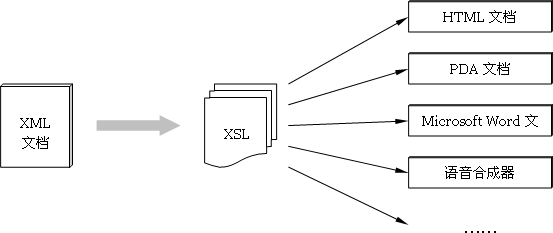
\includegraphics[scale=0.5]{xml_xsl.png}
\caption{可扩展样式表语言(Extensible Stylesheet Language,XSL)}
\label{xml_xsl}
\end{figure}

用XML规定的语言还有一个方便的特征,就是用这种语言的编写的文档可以轻松的自动生成。有些软件系统(通常具有底层数据库)可以用来生成大量易于在线传输和分析的数据,而生成的这些数据就能被转换成最适合每个用户浏览的格式。

有些组织为特定的主体开发了专用的XML,例如,化学家和化学工程师定义了化学标记语言(CML)以标准化分子数据的格式,CML包括大量有关化学的标记,给化学专业人员提供了共享和分析数据的通用格式。
	
XML是标记规约语言,XML文件则是数据。除非用户运行显示XML文件的程序(如浏览器),或者运行用它门进行操作的程序(如把数据转换成另一种格式的转换器或读取数据的数据库),或者运行修改它们的程序(如编辑器),否则什么都不会发生。


\section{XSLT}

XSLT(可扩展的样式表语言转换,Extensible Stylesheet Language Transformations),是用于转换 XML 的语言。

未来的网站将不得不向不同的浏览器并向其他web服务器以不同的格式传递数据。而 XSLT 则是一种将 XML 数据转换为不同格式的新的 W3C 标准。

XSLT 可以把 XML 文件转换为浏览器可识别的格式,比如 HTML,或者 WML - 一种用于许多手持设备的标记语言。

XSLT 还可以添加元素,并对元素进行删除、重新排列及排序,测试并确定显示哪些元素,等等。

	
XML和相关技术为信息管理和以各种方式在Web上有效地进行信息通信提供了强有力的机制。







\chapter{语义网}

“如果说 HTML 和 WEB 将整个在线文档变成了一本巨大的书,那么 RDF, schema, 和 inference languages 将会使世界上所有的数据变成一个巨大的数据库。” 

\begin{flushright}
——Tim Berners-Lee, Weaving the Web, 1999
\end{flushright}

$$\text{语义网(Semantic Web)}=\text{有意义的网络}$$

其中semantic(语义的)这个词指有意思的或与之相关的,语义网就是一种使用可以被计算机理解的方式描述事物的网络。

下面这样的句子可以被人类理解,但是怎样才能够被计算机理解呢?

\begin{compactitem}
\item 甲壳虫乐队是来自利物浦的著名乐队。
\item 约翰.列农是甲壳虫乐队的成员之一。
\item 唱片 "Hey Jude" 是由甲壳虫乐队录制的。
\end{compactitem}


陈述是由语法规则构建的,一门语言的语法定义了构建该语言的陈述所需的规则,这就是语义网的本质所在——以计算机应用程序可以理解的方式描述事物。



语义网和网页之间的链接没有关系,语义网描述的是事物之间的关系(比方说 A 是 B 的一部分,而 Y 是 Z 的成员)以及事物的属性(例如尺寸、重量、使用期限和价格等等)。

\section{语义网技术}

语义网不是快速发展的技术,RDF(资源描述框架,Resource Description Framework)是一种用于描述网络上的信息和资源的的标记语言,语义网使用 RDF 来描述网络资源。

RDF 是由那些拥有逻辑学和人工智能方面的学院背景的人们发展起来的。对于一般的开发人员的来说,它并不是特别容易被理解,其中,RSS就是一种用于构建语义网应用的快速发展的语言。

将信息置于RDF文件之中,这样的话,这些信息就有可能被计算机程序("web spiders")从网络中搜索、发现、收集、筛选、分析和处理。


举例来说,假如有关音乐、汽车、入场券(或者任何别的东西)的信息被存储于 RDF 文件,智能网络应用程序就会将信息从不同的源中进行收集,并将其整合,然后以一个有意义的方式将信息提交给用户们。


类似如下内容的信息:

\begin{compactitem}
\item 不同经销商的汽车价格
\item 药品信息
\item 航班时刻表
\item 工业备件
\item 书籍信息(价格、页数、编辑、年份)
\item 某人是谁
\item 事件的日期
\item 软件更新
\end{compactitem}


语义网不是可供搜索的免费文本,如果希望搜索或访问语义网,我们需要软件的协助。

要使用语义网,我们就需要 “语义网代理”(Semantic Web Agents)或 “语义网络服务”(Semantic Web Services),这些“代理”或“服务”会帮助我们在语义网上找到正在寻找的东西。

在语义网上,我们可能会搜索这些信息:

\begin{compactitem}
\item 最便宜的机票
\item 适合我的汽车的装饰
\item 书籍、电影或音乐
\item 天气预报
\item 时间表和日程
\item 股票价格和汇率
\end{compactitem}

在未来,要想在 Web 上找到任何信息,也许使用“语义网代理”就可以了。


\section{语义网安全}

用户的疑问是:“我能信赖语义网上的一个卖家吗?我能信任语义网上的一个买家吗?”。要解决上述问题,就需要访问更多 RDF 文件:

\begin{compactitem}
\item 信用卡信息
\item 银行信息
\item 语义网记录
\item 社会安全信息
\end{compactitem}


\begin{longtable}{|p{90pt}|p{90pt}|p{90pt}|p{90pt}|}
%head
\multicolumn{4}{r}{}
\tabularnewline\hline
Source	&Person ID	&Person Name	&Status
\endhead
%endhead

%firsthead
\hline
Source	&Person ID	&Person Name	&Status
\endfirsthead
%endhead

%foot
\multicolumn{4}{r}{}
\endfoot
%endfoot

%lastfoot
\endlastfoot
%endlastfoot
\hline
Citybank			&11223344	&Jim Green	&trustworthy\\
\hline
VISA				&11223344	&Jim Green	&trustworthy\\
\hline
Recorded			&11223344	&Jim Green	&unknown\\
\hline
US Social Security	&11223344	&Jim Green	&born 10-10-1984\\
\hline

\end{longtable}

通过使用类似的这些 RDF 文件,“语义网”代理就能够确定能够我们是否能信任正在打交道的这个人(能够通过 eBay 和 Amazon 之类的因特网交易公司来提供记录信息)。

\section{语义网支付}



要运营语义网,就必须开发支付手段,而易用的因特网“储蓄存款”可能成为此问题的解决方案。

“储蓄存款帐户”是一种只能接受存款的帐户。它可以为因特网上的所有提供便利,只要得到用户的 ID(或者电子邮件地址,很类似 PayPal),任何人都可以把钱存入指定的帐户。

通过使用这种支付手段,每个人都可以在因特网上公布他们的银行帐户,并在不需要中间人的情况下出售他们的汽车,这可能是未来的因特网银行的样子。

以后,用户需要卖一本书的情景可能如下:

\begin{compactitem}
\item 打开 OWL 代理
\item 在种类中输入 “Book”
\item 在新窗口中填写关于书的信息
\item 填写印在书上的 ISBN 号码
\item 选择“二手”,以及 "condition as new",并单击返回
\item OWL 代理会自动填写其余的部分
\item 作者、年份、页数... 现在所有的信息都完整了
\item OWL 代理已经搜集好您需要出售的书籍的所有信息
\end{compactitem}

最后,用户点击拍卖按钮。而对于“拍卖代理”,执行的动作可能是:

\begin{compactitem}
\item 拍卖代理打开了。
\item 用户填好了最低价格,然后点击“提交”。
\end{compactitem}

这样,用户的书籍就可以在因特网上进行拍卖了。


\section{语义网应用实例}


假设某个语义网系统用于通过因特网管理二手车的销售和购买,该系统可能包括两个主要的应用程序,其中一个针对希望购买汽车的人群,另一个针对希望出售汽车的人群。这里把这两个应用程序称为 IBA (I Buy Application) 和 ISA (I Sell Application)。

希望购买汽车的人群使用的 IBA 应用程序类似这样:

\begin{figure}[!h]
\centering
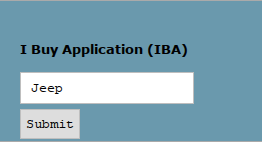
\includegraphics[scale=0.5]{semantic_web_example_buy.png}
\caption{IBA}
\label{semantic_web_example_buy}
\end{figure}


在真实世界的应用程序中,买方可能在第一次使用该程序时被要求标示自己的身份,然后买方的 ID 将存储在一个 RDF 文件中,ID 会把买方标示为一个带有名字、地址、电子邮件以及 ID 号的人。

当买方提交查询后,应用程序会返回一个待售汽车的列表,这个列表会按照年份、价格、位置和可用性进行排序。通过Web对 RDF 文件的搜索,此信息会不断地从 web spider 返回。

希望出售汽车的人群使用的 ISA 应用程序类似这样:

\begin{figure}[!h]
\centering
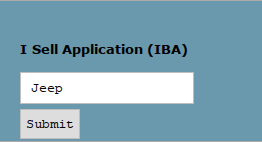
\includegraphics[scale=0.5]{semantic_web_example_sell.png}
\caption{ISA}
\label{semantic_web_example_sell}
\end{figure}


当卖方提交表单时,应用程序会向卖方请求更多的信息(包括年份、价格、位置等),并把卖方的 ID 和信息存储在一个 RDF 文件中,以供Web使用。

RDF 文件包含的信息类似:

\begin{compactitem}
\item ID:姓名、地址、电子邮件、ID 号等
\item 需求条目:名称、型号、价格等
\item 出售条目:类型、型号、图片、价格、描述等
\end{compactitem}

在幕后,这个 "ISA" 应用程序会创建一个带有许多 RDF 指针的 RDF 文件,RDF 指针是一种指向有关某事物的信息的指针(实际上是 URL),类似知识数据库。

比如,它会创建一个指向带有关于 person 信息的文件的指针,一个指向带有关于 Volvo 和 Volvo 型号信息的文件的指针,一个指向带有关于 Volvo 经销商和出售者信息的文件的指针,等等。


有关于此的优点在于用户不必对自己本人或汽车的型号进行描述,而这个 RDF 应用程序会为用户对信息进行整理。


RDF 是关于数据的数据 - 即元数据,RDF 文件经常会描述其它的 RDF 文件。将来有可能把所有的 RDF 文件连接起来构建一个语义网吗?没有人知道,但是总有人去尝试。


我们不认为语义网会依靠自己发展起来。它需要第三方的协助才能成为现实。不太可能的是,用户仅仅在因特网上发布 RDF 文件,就能够出售自己的汽车。

必须通过很多力量的参与,才能够发展类似上面的 "ISA" 和 "IBA" 应用程序。一方为所有的项目构建搜索引擎数据库,另一方则为其开发标准。可能是 eBay,或 Microsoft,或 Google,也可能是别的公司,但是总会有人去做。


或许有一天,用户将能够使用标准化的 RDF 文件在 Web 上收集有关几乎所有事物的信息。它可能免费,但也可能不得不为信息来付费,但在因特网上发布信息将比过去更加容易。





\bibliographystyle{plainnat}
\bibliography{csnotes}
\clearpage








